\begin{landscape}
% \savegeometry{original}
\newgeometry{a4paper, bottom=2.54cm}
\begin{adjustbox}{minipage=\linewidth}
% \hspace*{-40cm}
\chapter{Design}
\vspace{-1.5cm}\section{Systems Diagram}
\begin{figure}[H]
    \vspace{-0.5cm}\includesvg[width=21cm]{ch2_design/systemsdiagram.svg}
    \vspace{-0.5cm}\caption{Systems diagram for the project}
    \label{fig:sysdiagram}
\end{figure}
\end{adjustbox}
\restoregeometry
\end{landscape}

For the systems diagram, I choose to decompose the program first into 3 global subheadings for the program. It bases off that the user will be accessing the landing page in order to login or sign up for the site or that they are on the homepage and are following one of the actions from that page. If a procedure is not needing its own page or is not going to be shown to the user, then it was placed in the maintenance section. 
Under the landing page section, we have the login and sign-up pages which consist of all the steps that either the system or the user will do in order to be able to gain access to the main website and access its features. The steps chosen aim to reduce the amount of work that the user will have to do to enter the site. 

With the home page section and more specifically the create a listing section there are a large number of procedures attached to it in order to ensure that a listing is fully completed. This has the intention of increasing the quality of listings on the site and aims to make sure that the buying experience is as good as possible for the user and aims to reduce the problem of having listings that don’t contain enough information about the camera. The search box page section contains everything that the user will need in order to be able to search for a camera on the page. It makes sure that if the user does select a listing, then all the information both on that specific listing and the camera itself are fetched from the database which ensures that the listing will appear as intended for the user. For the price recommendation page, it aims to be as simple as possible and so returns results quicker. The sign out procedure only requires one step as to sign a user out they are returned to the landing page where they will have to sign back into the page.

In the maintenance subheading, it contains all the procedures that the user won’t see. The updating the price recommendation will work whenever a listing ends meaning it will not run the code unnecessarily. By choosing to just take a mean of the values that various listings of the same cameras have sold for, it makes the price recommendation more accurate for the website specifically. This matches the designed use of the tool in that it is used in tandem with selling on the website rather than for use in tandem with other websites. The listing ending procedure will ensure that the site runs properly and that listings are properly over when the timer for them has ran out. The process also incorporates the steps that are required in order to notify, through email, the seller and winning bidder that they have won their item. Finally, the bidding on a listing works to ensure that when the user enters a bid, it complies with the requirements. It also will work to keep the database updated in order that other users who view the auction at a later date get the most up to date information of what the price of the auction is. 

\section{Proposed screen designs and usability features \parencite{wireframe_cc} \parencite{hewer}}
\subsection{Landing page}
\begin{figure}[H]
    \centering
    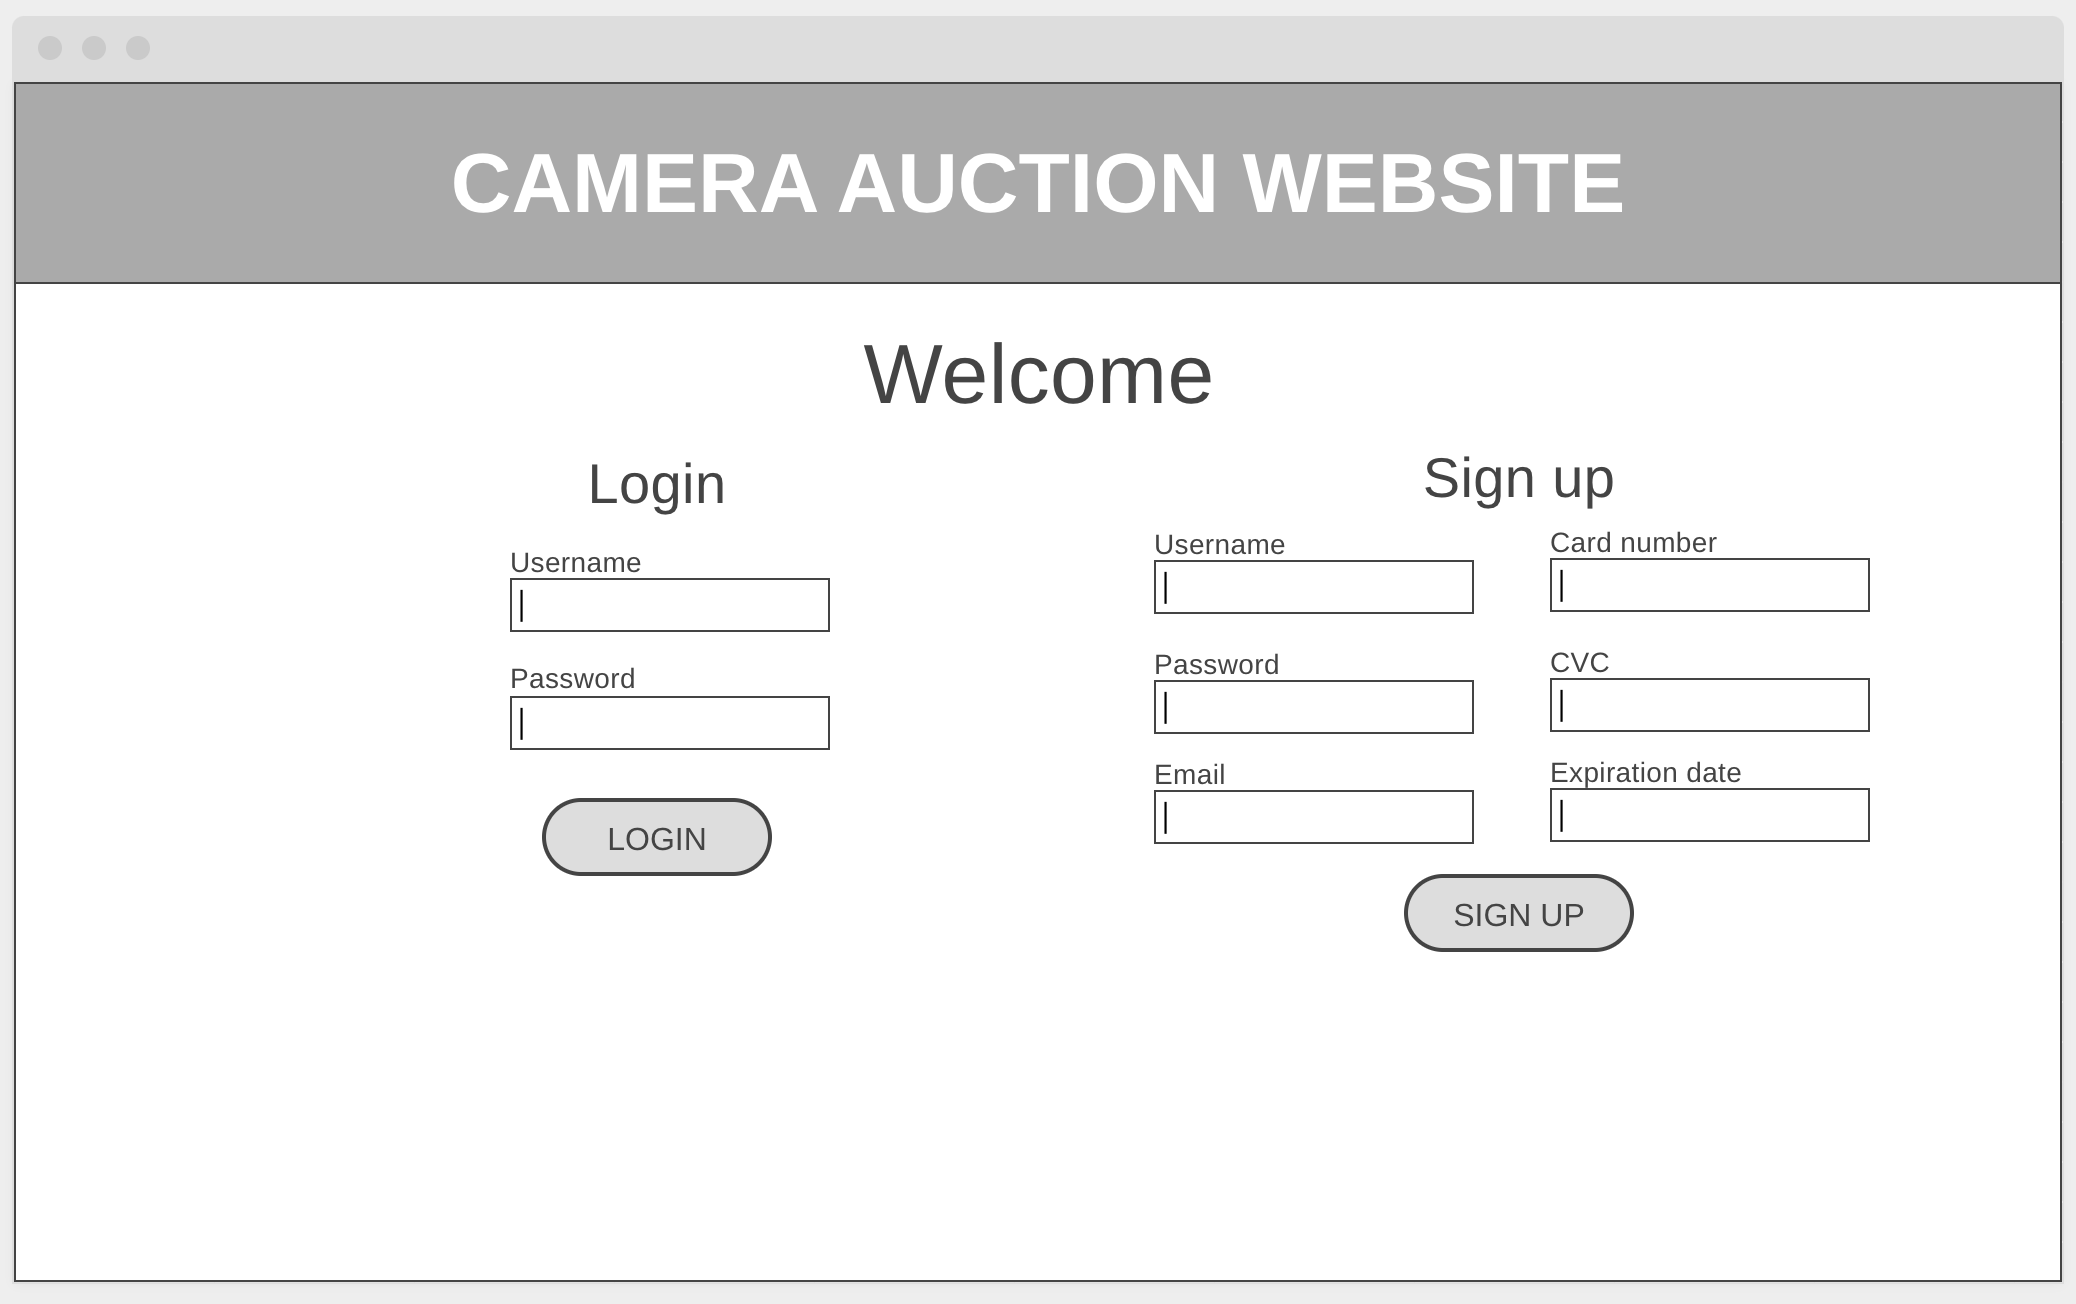
\includegraphics[scale=0.35]{ch2_design/wire_landing.png}
    \caption{Landing page design}
    \label{fig:wire_landing}
\end{figure}
The landing page has been designed as so in order to best allow the user to quickly access the auction website. By having all the forms required on a single page, it reduces the number of interactions that the user will need to have with the system before being able to actually use the site as intended. The forms are all labelled with larger text in order to guide the user so that they don’t attempt to sign up to the webpage through a login form which would result on not all the relevant information being stored on the user and thus the site not working as intended. The distinction of the actual submit buttons through the bolder ring, which creates a ‘pop-out’ effect, directs the users attention to them meaning that they are not left confused about which button they should be pressing.

\subsection{Home page}
\begin{figure}[H]
    \centering
    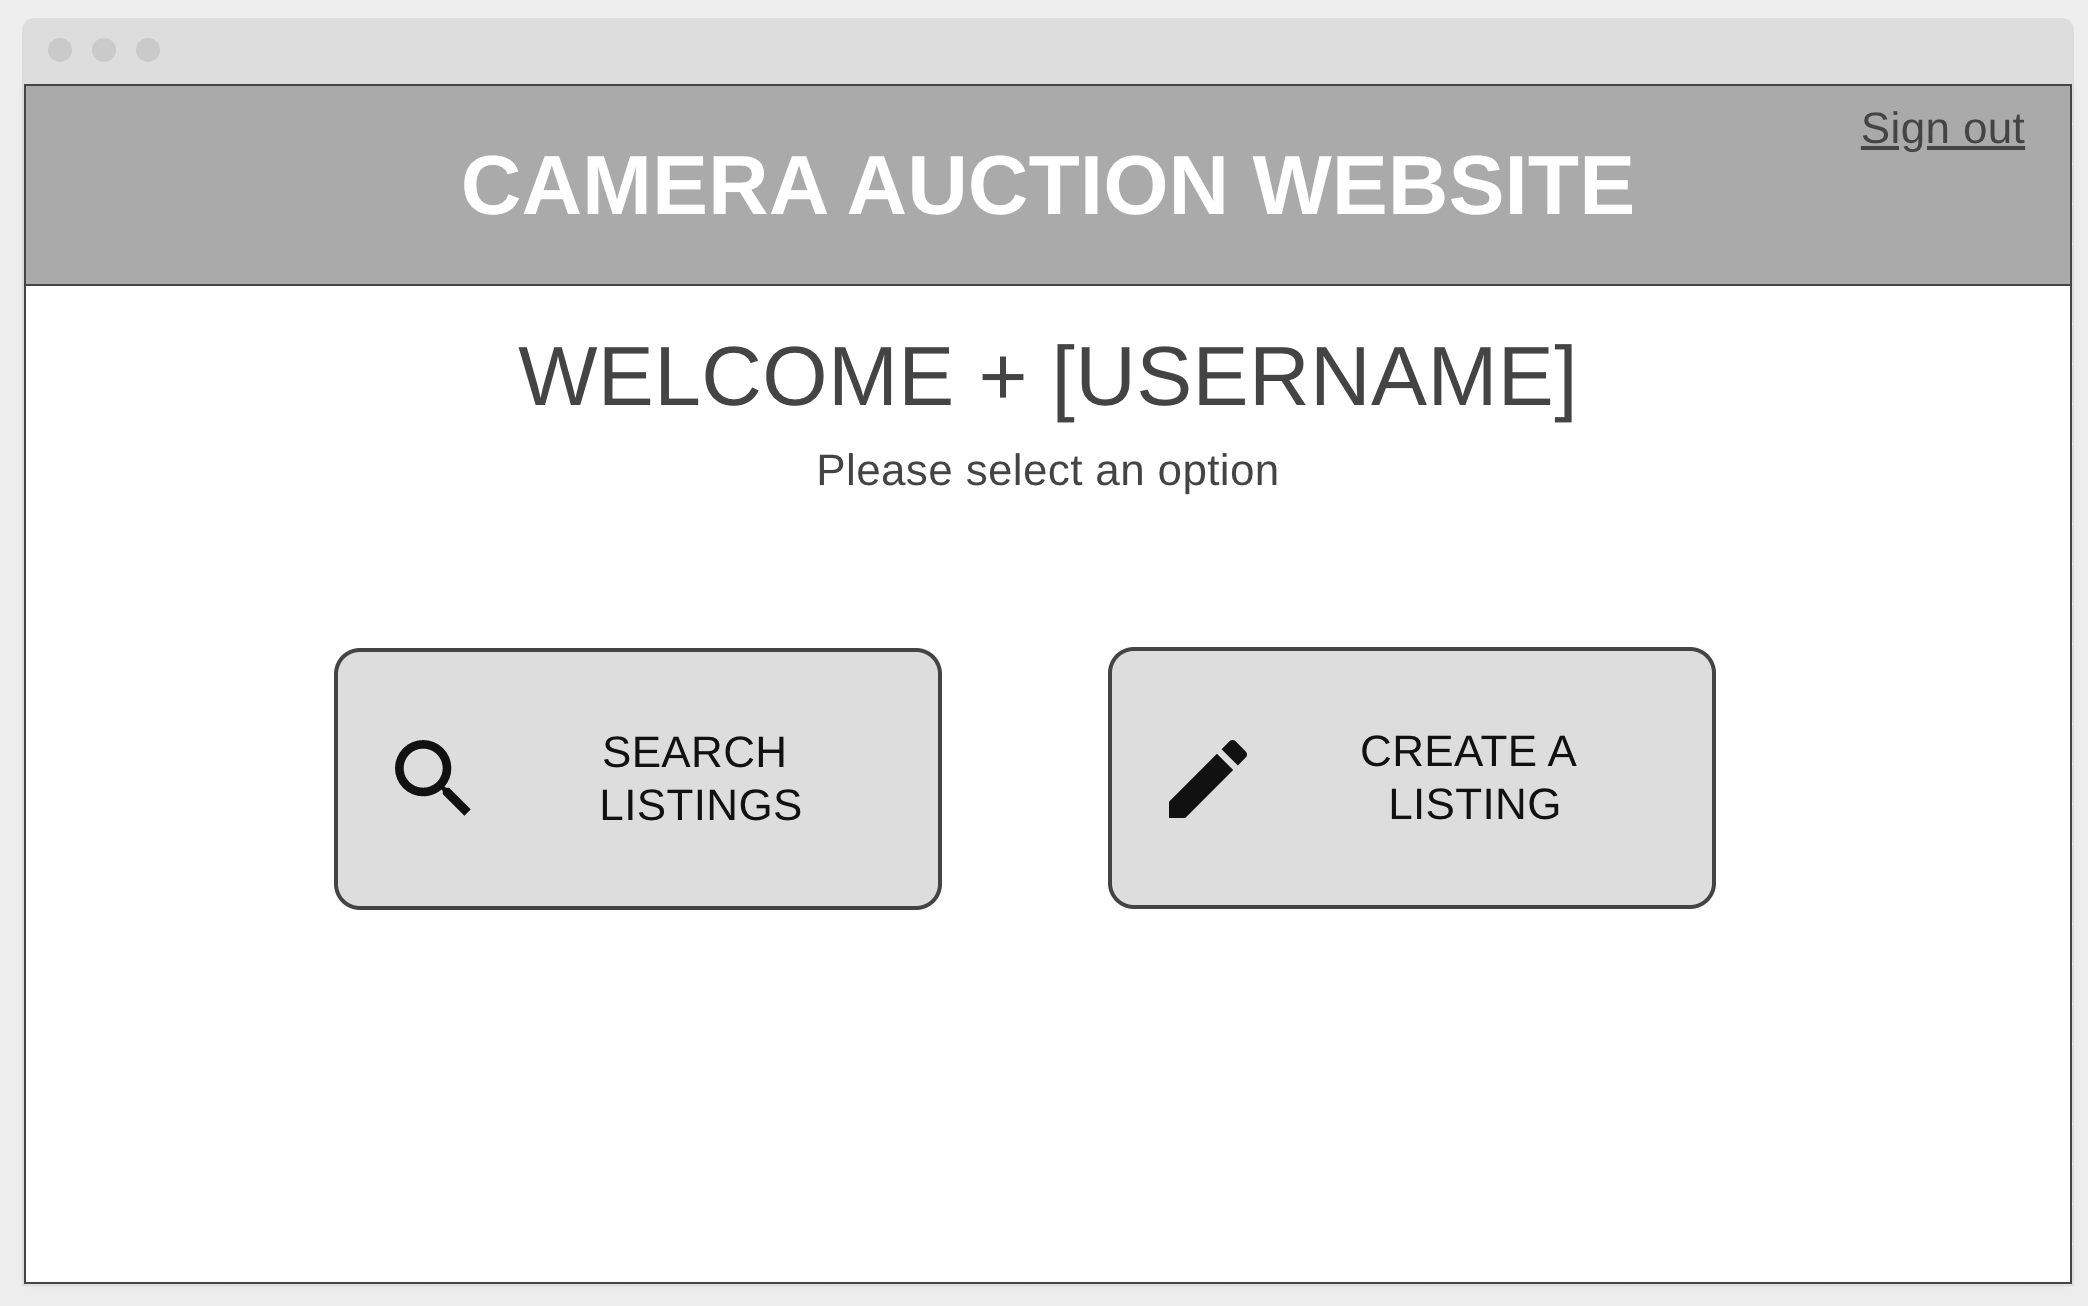
\includegraphics[scale=0.4]{ch2_design/wire_home.png}
    \caption{Home page wireframe }
    \label{fig:wire_home}
\end{figure}
The home page has a single design that makes it clear to the user what their options are when they are on the page. These large buttons will grab the user’s attention when they enter the page and allow them to progress to their desired action as quickly as possible. The use of icons for the buttons makes them more universal to people and offsets the amount of text that is on the page. The buttons are in the same style as the landing page which the user should have come from and thus maintains continuity, which is one of the Gestalt’s laws, across the webpage.

\subsection{Search page}
\begin{figure}[H]
    \centering
    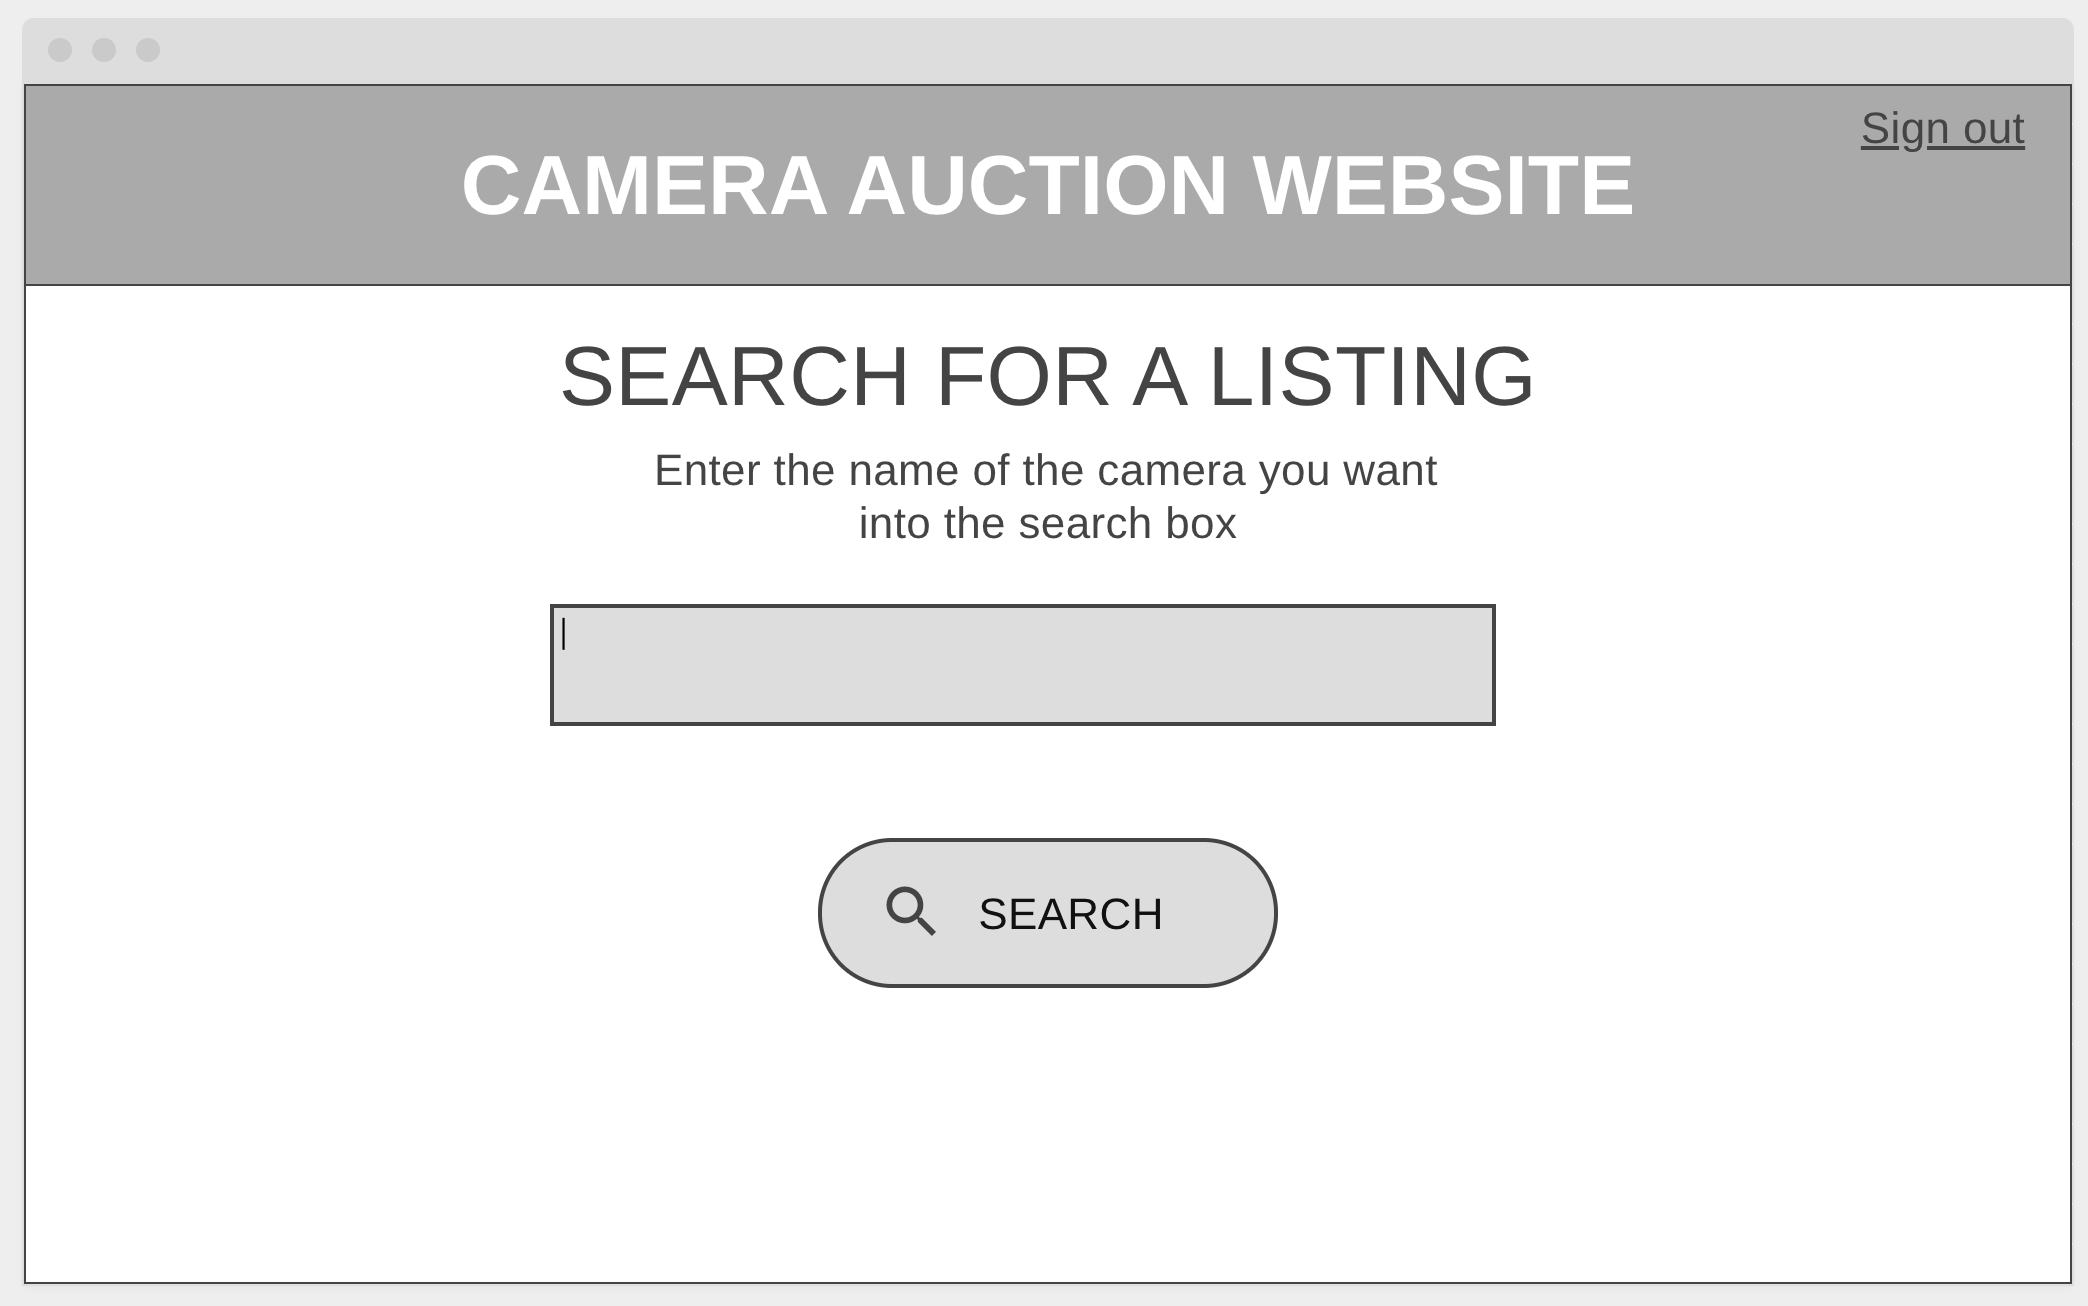
\includegraphics[scale=0.4]{ch2_design/wire_search.png}
    \caption{Listing search wireframe}
    \label{fig:wire_search}
\end{figure}
The search box page consists of two main elements, a large text field and a large search button. This reduces the complexity of the page and draws the user to main item on the page, the large textbox. The search box is then followed by the search button which is the same style as previous buttons and uses the same icon from the landing page before which all ensures continuity across the site.

\subsection{Search results}
\begin{figure}[H]
    \centering
    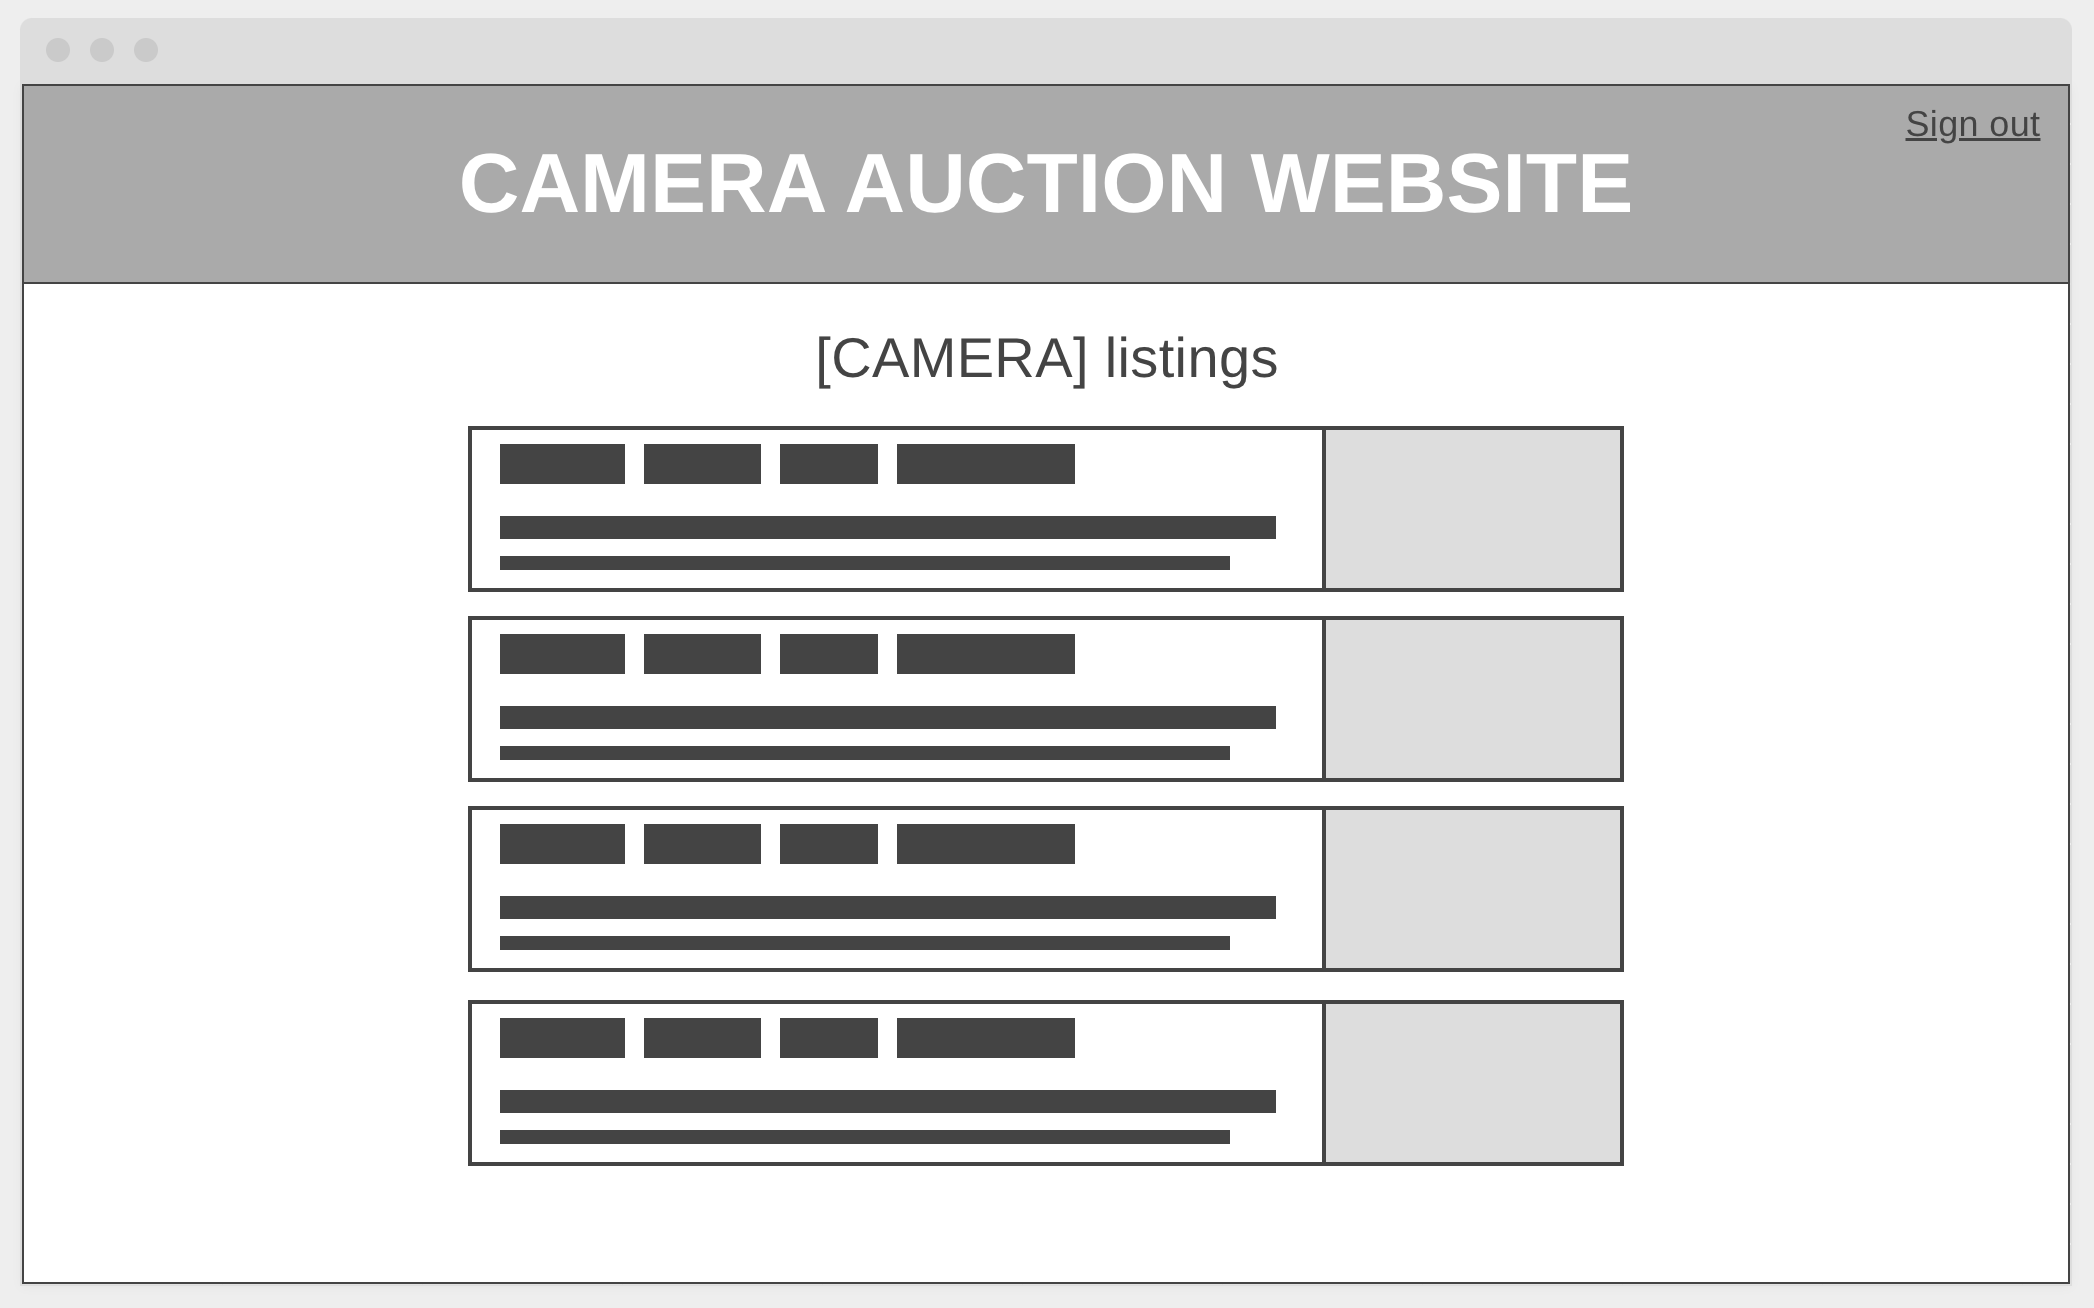
\includegraphics[scale=0.4]{ch2_design/wire_listings.png}
    \caption{List of auctions for a camera wireframe}
    \label{fig:wire_results}
\end{figure}
Each of the boxes returned on the page represents one listing from the database. The boxes ensure a distinction between which listing is which and which information matches the specific camera. For each of the boxes, it contains a large, eye-catching title which will clearly show the user what make and model the camera is. Along with this, the return will contain a short description of what the item is or what the listing contains. This decision aims to improve the site experience by making it easier to decide between listings without having to delve into each listings specific page. Each listing block will also contain the first image for the listing which helps the user to get a brief idea of what the camera is in and spot any listings that are in particularly bad condition.

\subsection{Camera Listing}
\begin{figure}[H]
    \centering
    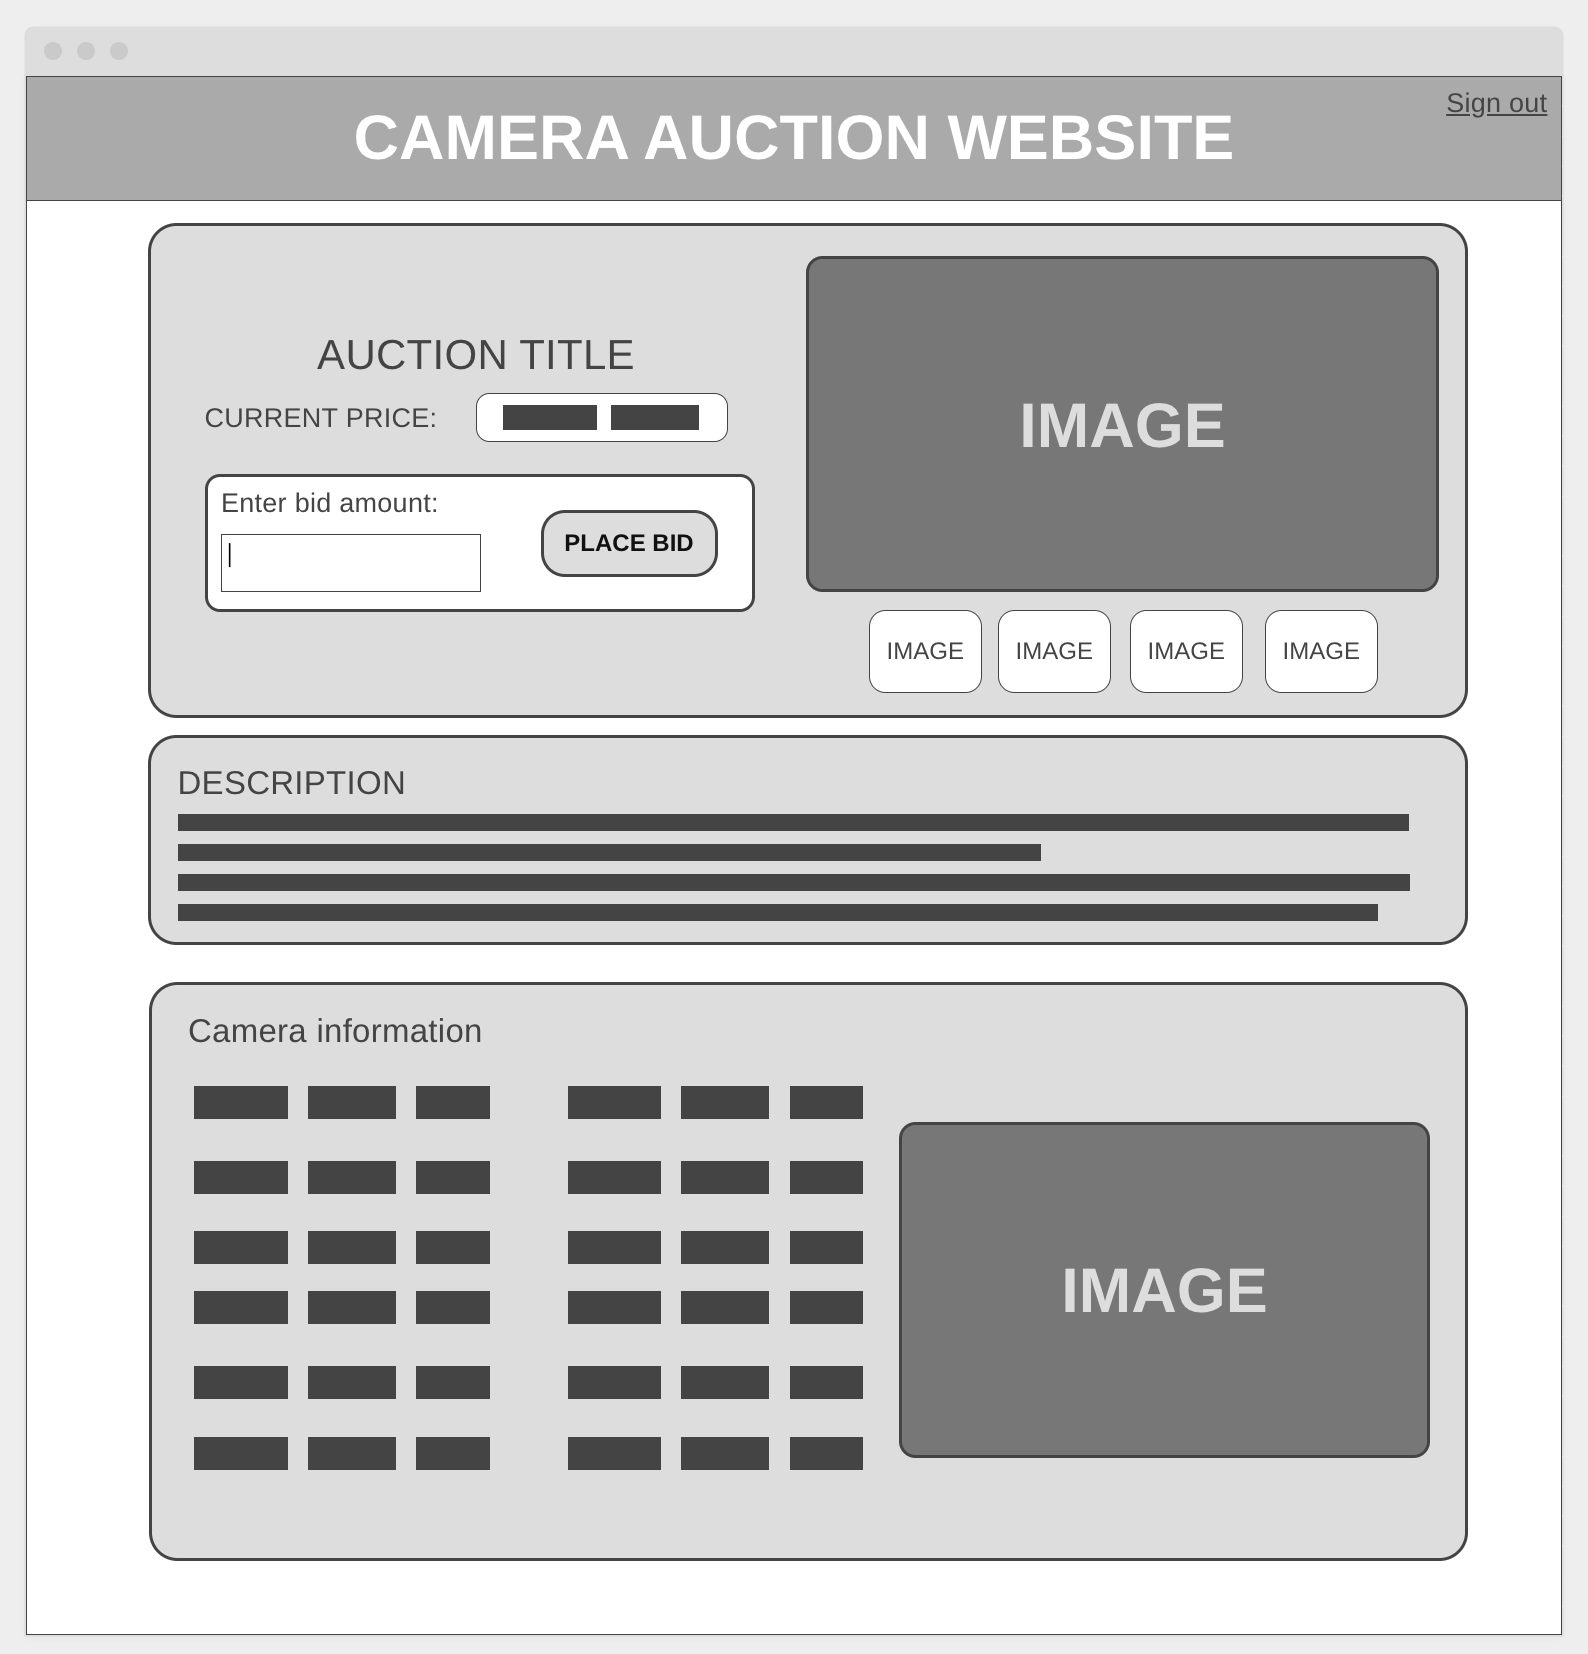
\includegraphics[scale=0.4]{ch2_design/wire_exlisting.png}
    \caption{Camera specific page wireframe}
    \label{fig:wire_listing}
\end{figure}
This is the main page that a user will use in order to bid on a listing. All the information is arranged into large boxes which aims to create distinction between the items on the page and helps to show the user what items are from the seller, such as title and description, and what items are from the system, such as the camera information. The page will include a large auction title in order to ensure that the user can confirm they clicked on the intended listing. The bidding box and current price are in a separate colour will also help to draw the user’s eye to it and thus encourage them to place a bid on the item. It contains a simple text box for the user to enter their bid and a submit button which will run the corresponding bidding procedure and will allow the bid to be added for the listing. The main image next to the bidding box will be the same image that the user saw on the search results page and will have the subsequently uploaded images shown below it in a carousel which the user can click through by clicking on the image. Below the first main box, is the description of the item which the user would have had to enter for the bid to be added to the site. The design is simple as to not draw focus away from the use when they are reading the information as it may be important to the user. Finally, there is the information section on the camera, this will be shown through a grid of headings and the corresponding answers. This section is naturally going to be less visually appealing to the user and so to counteract this, I decided to include a large generic image of the camera in order to break up the text. 

\subsection{Price prediction}
\begin{figure}[H]
    \centering
    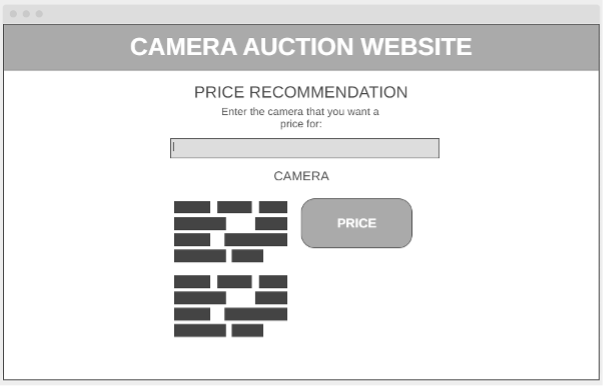
\includegraphics[scale=0.7]{ch2_design/wire_price.png}
    \caption{Price recommendation page wireframe}
    \label{fig:wire_page}
\end{figure}
The price recommendation screen allows the user to retrieve an average price for the listings that have been sold on the site. It allows the user to search for a camera against the database of camera information. The query will then output the information about the camera, as shown with the blocks on the left hand side along with an overall price displayed boldly on the right hand side. This allows for the user to clearly see what the price of the sold listings are for that camera. The display of camera information is also with the aim of allowing the user to ensure that they have retrieved the camera that they wanted.  

\section{Key processes \parencite{microsoft_visio}}
\subsection{Login verification system}
\begin{figure}[H]
    \centering
    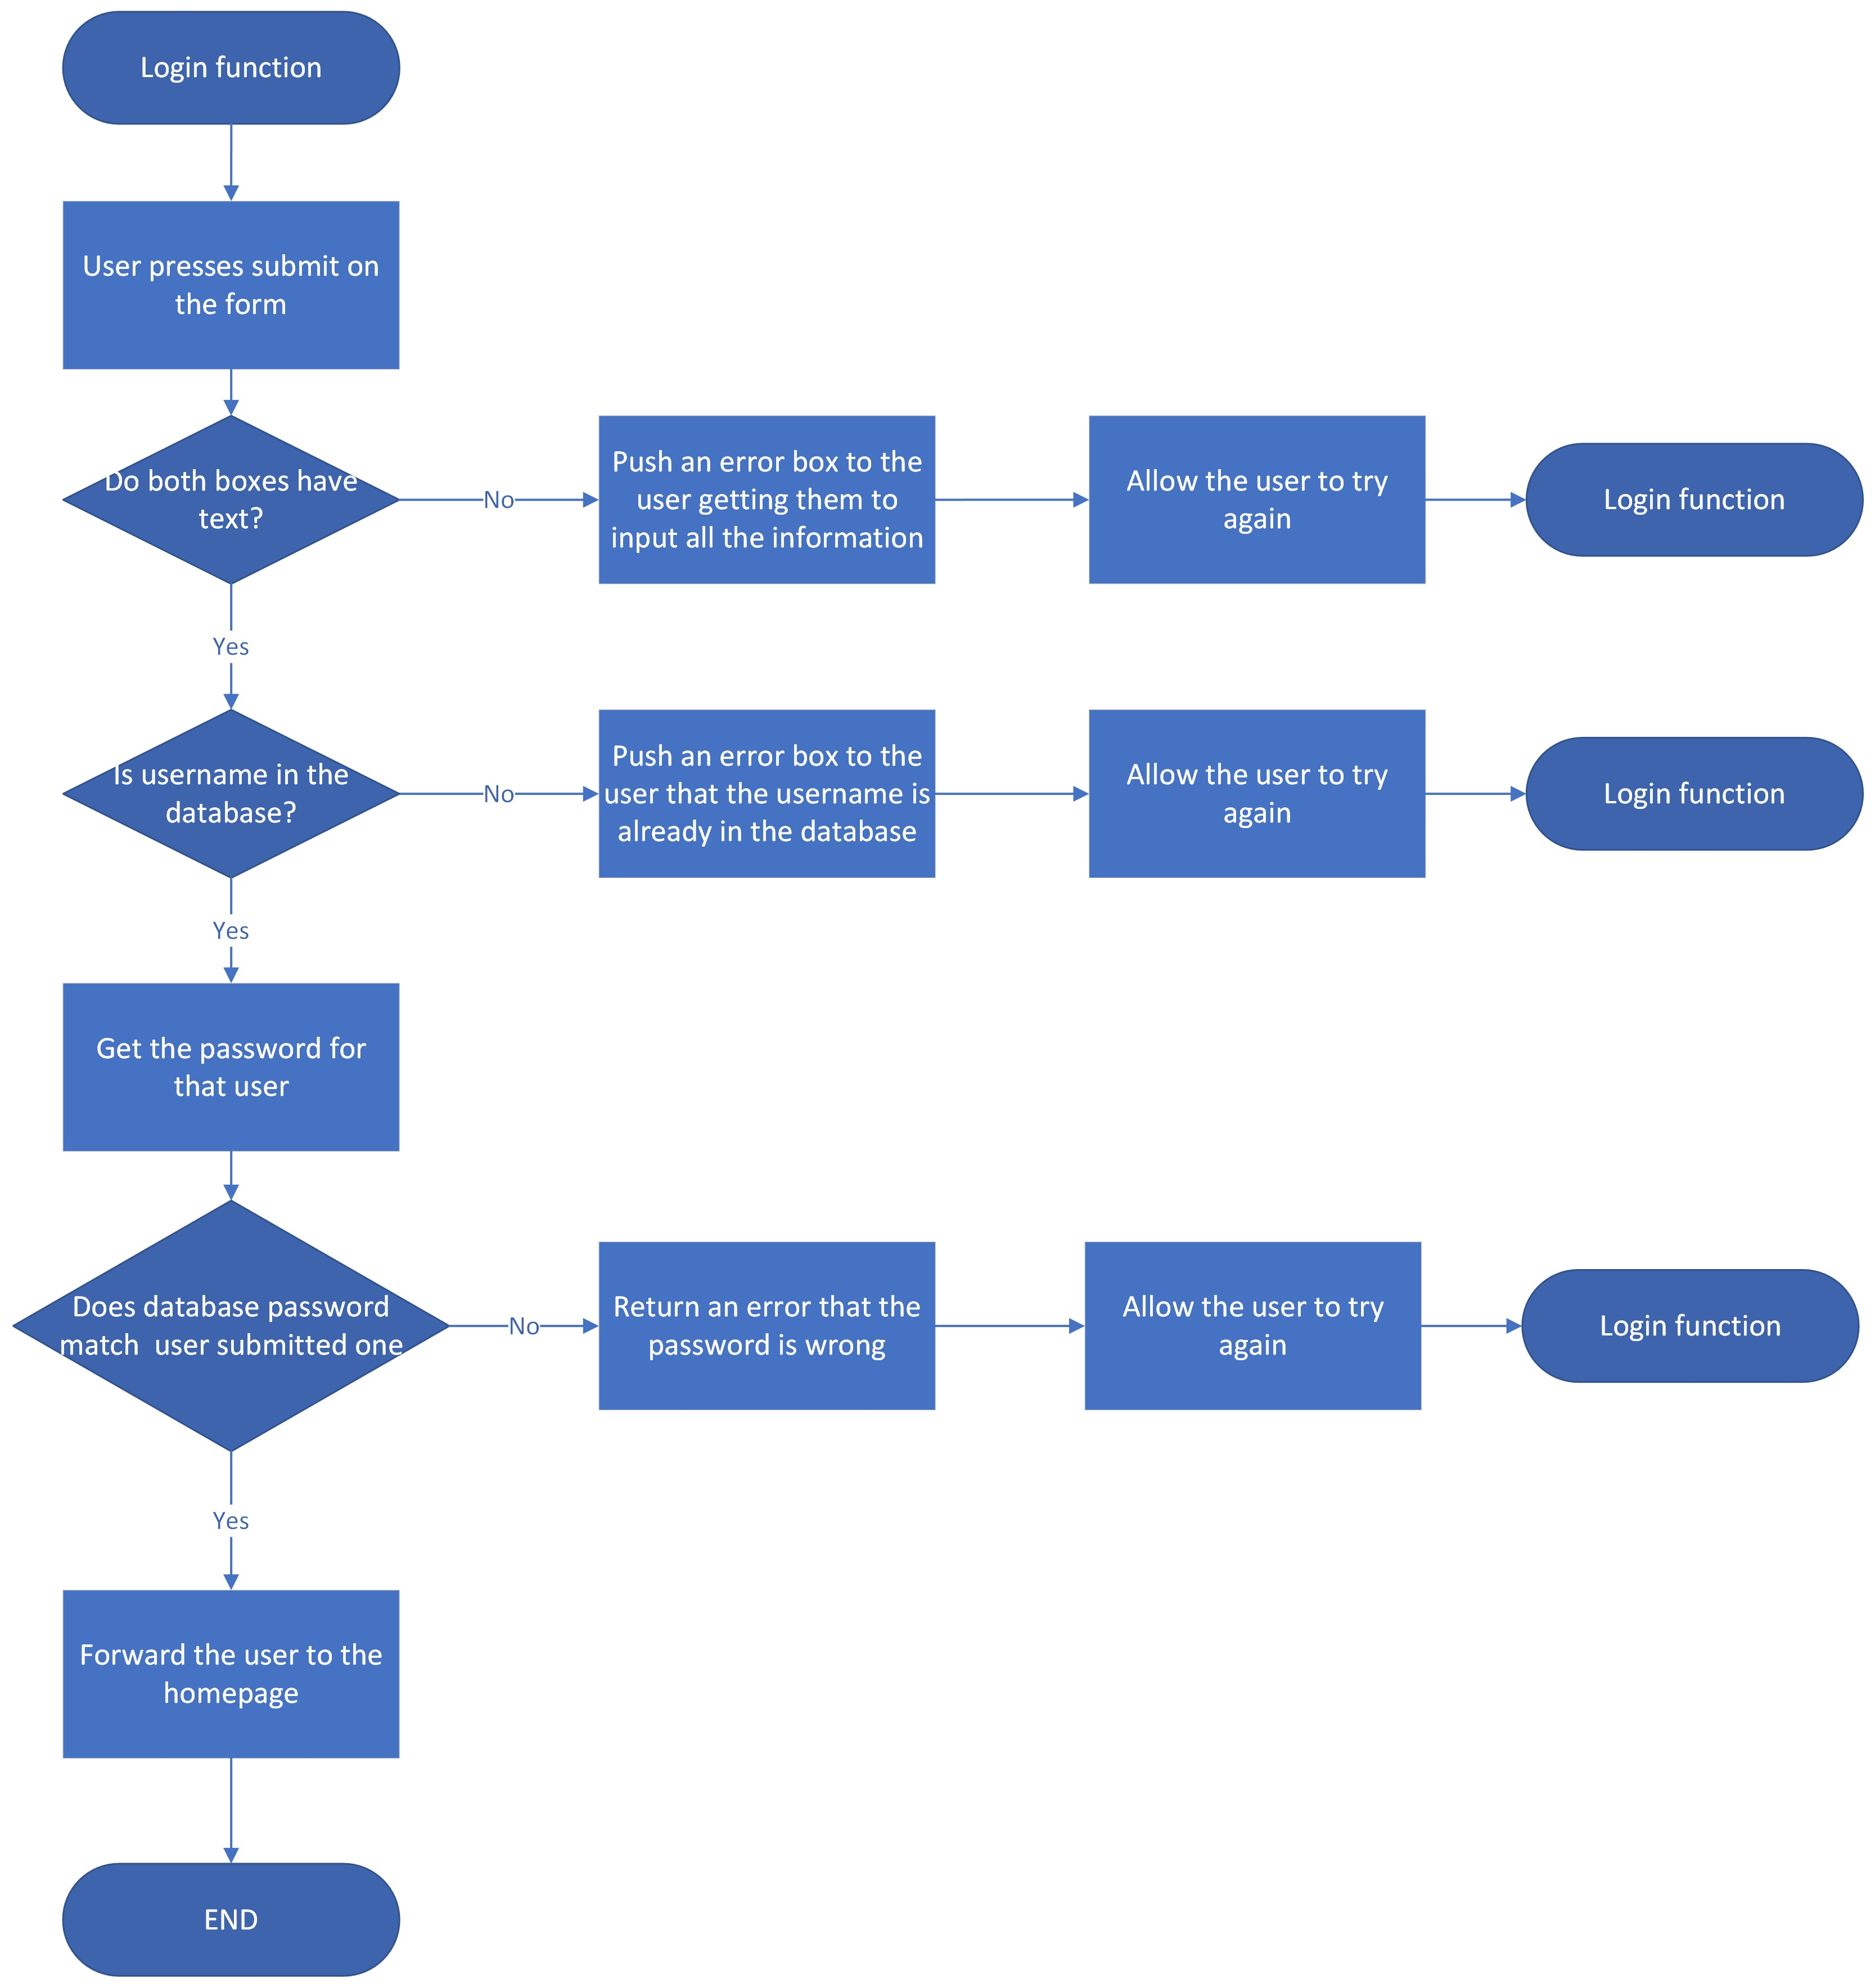
\includegraphics[scale=0.2]{ch2_design/c3_login.jpeg}
    \caption{Flowchart for login verification system}
    \label{fig:flow_login}
\end{figure}
The process will work through the process of first ensuring that the user has entered information into the form in order to ensure that the rest of the procedures for verification of the details runs smoothly. Should there not be all the information entered, they the user will have an error returned stating that all the information is not filled in. This then leads to the username being checked to see if it is in the database itself. I’ve chosen to check with username since it should be unique and there should not be any clashes with multiple people having the same username. There is also an error should the username not be found to let the user know the username is not valid. Finally, the password is fetched from the database and compared to the password the user has entered and providing the two matches, then the user is redirected to the homepage in order to access the site.

\subsection{Sign-up verification system}
\begin{figure}[H]
    \centering
    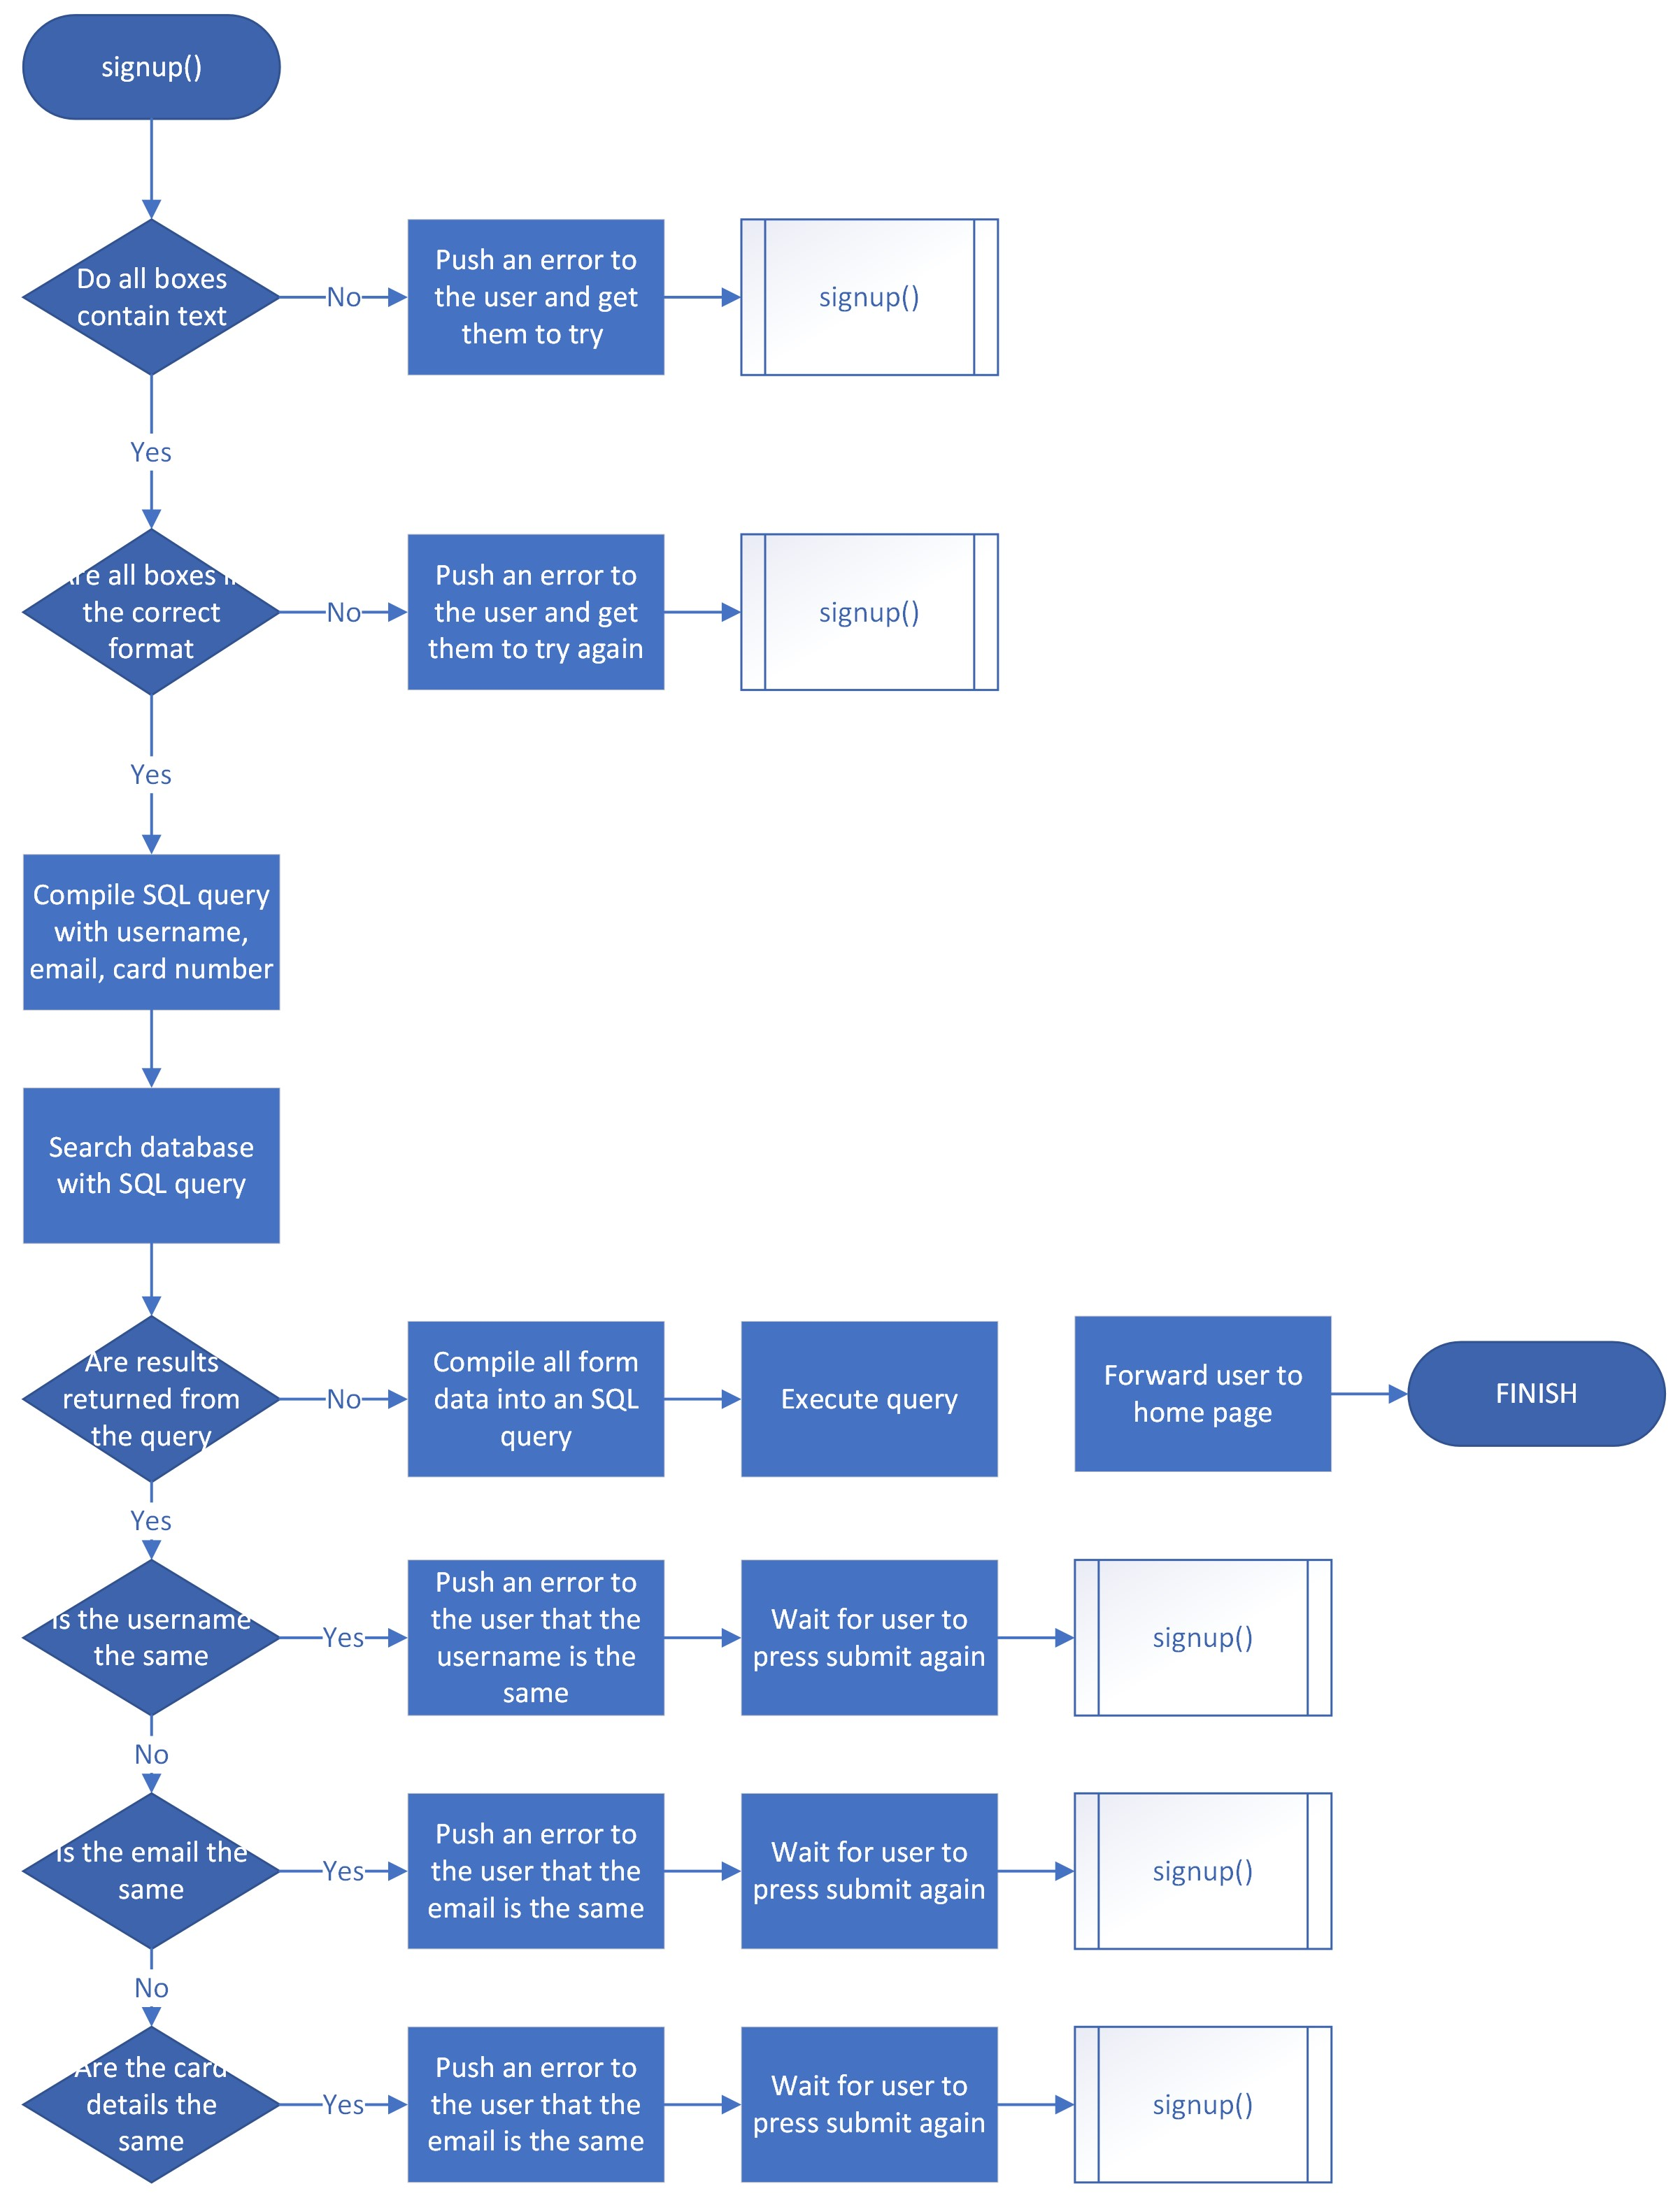
\includegraphics[scale=0.3]{ch2_design/c3_signup_2.jpeg}
    \caption{Flowchart for sign-up sub-process}
    \label{fig:flow_signup}
\end{figure}
 The sign-up system will first ensure that the user has filled in all the boxes. This is to ensure that the rest of the procedure has no issues when it comes to getting results as not having anything to query with will mean that no duplicate results can be returned which would mean that duplicate details could be added to the database. The following step to ensure that each box is in the correct format is to guarantee that the SQL query will not have any issues of writing data when it comes to submitting the user’s details which could be caused from inputs being in the wrong format. I felt the simplest way to search for duplicate details would be to use the details entered to the form as the search terms. The program will search the database for any results that are returned from the queries. By then comparing the queries that are returned to see what is duplicate, the user will be notified of what is duplicate and can remove the specific item.

 \subsection{Listing search}
 \begin{figure}[H]
     \centering
     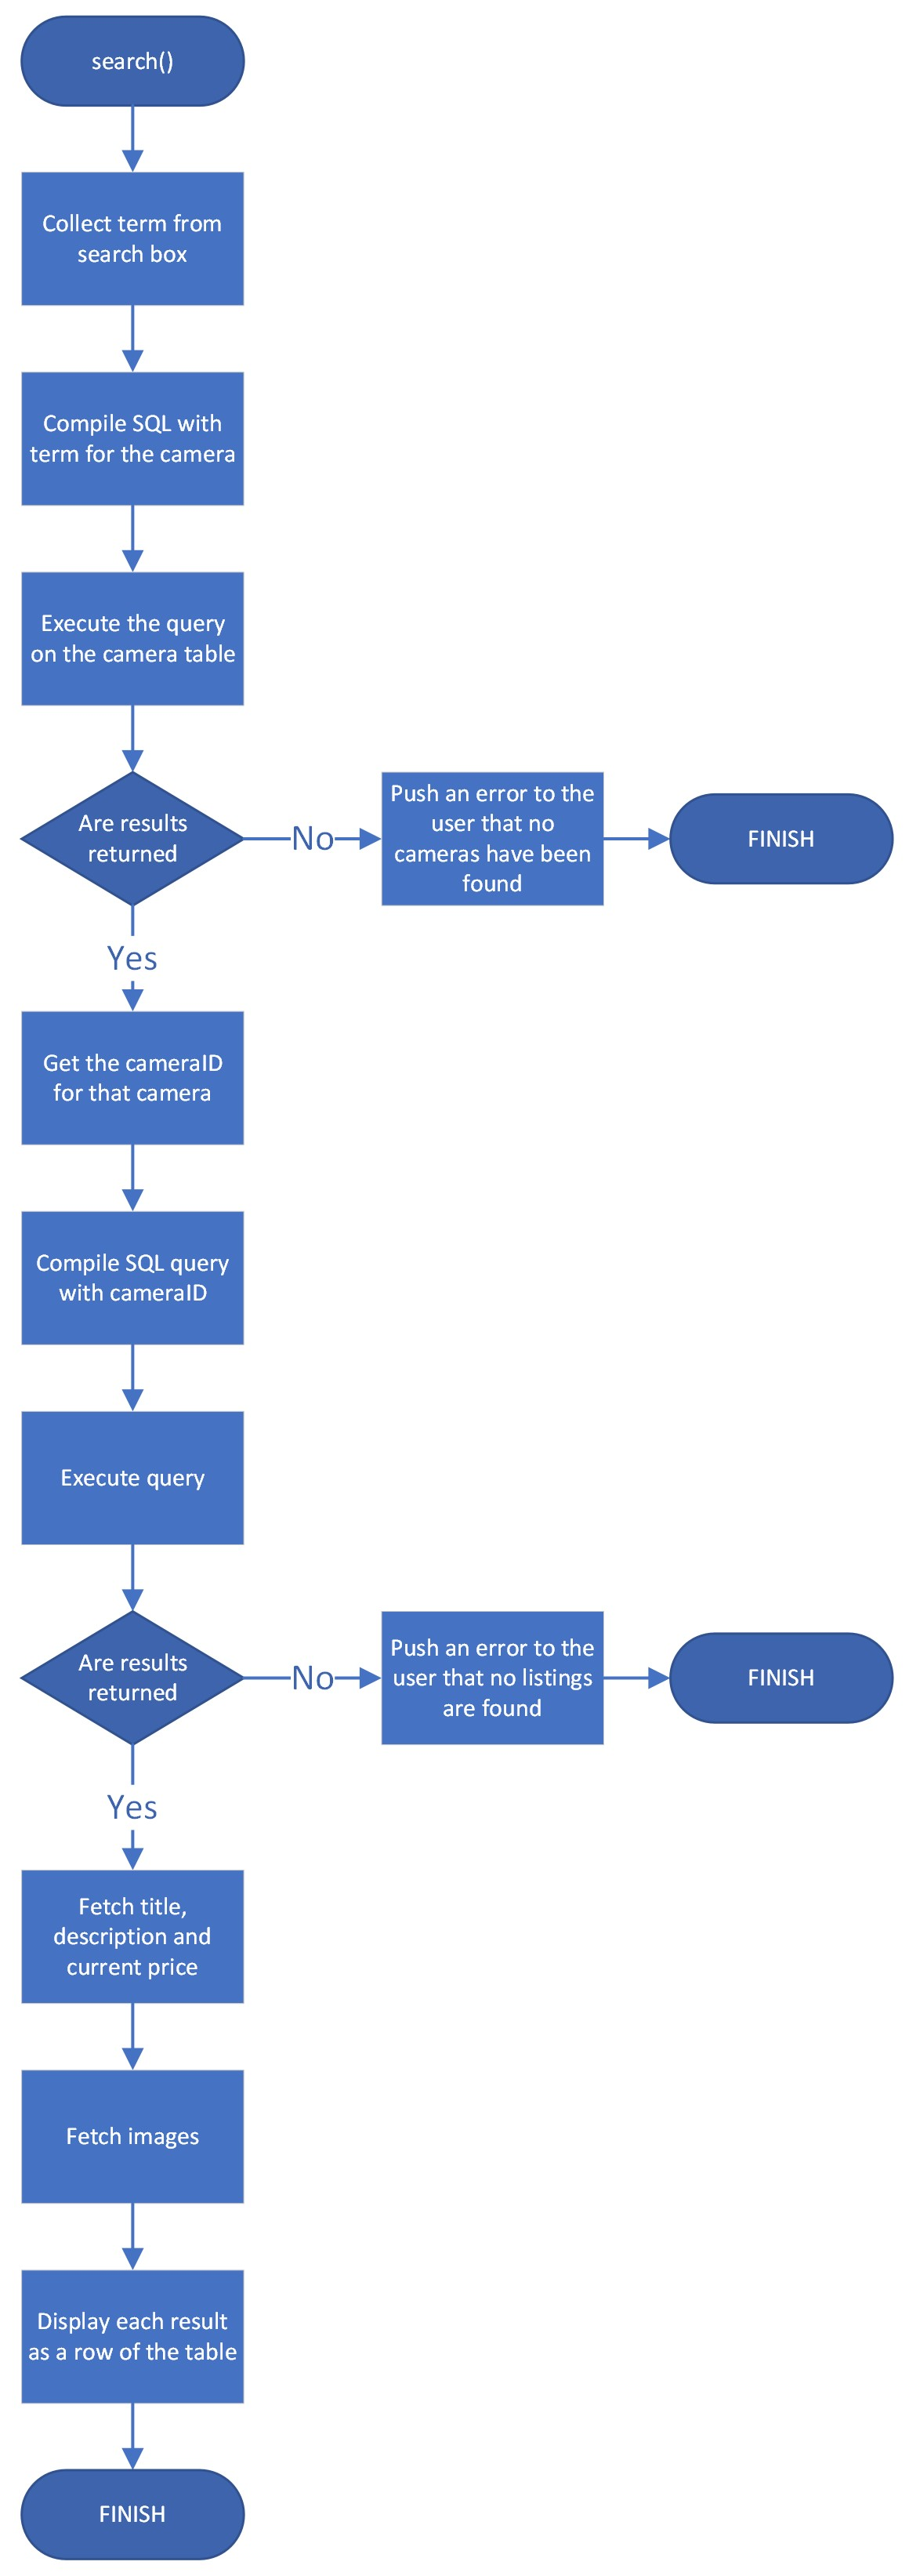
\includegraphics[scale=0.3]{ch2_design/c3_search2.jpeg}
     \caption{Flowchart for the listing search sub-process}
     \label{fig:flow_search}
 \end{figure}
 The camera search flow chart will work by taking the camera that the user enters and using that to find the id for each specific camera. This ID will act as the primary key across the database tables for each camera. With this in mind, it enables this reduces the risk of having camera names in different formats across the table and so by using ID it can be sure to of no issues. At this stage, I decided to only return the title, price and description in order to reduce loading times on the page. By displaying the listings in a table, it makes all the listings accessible to the user.

 \subsection{Create a listing for the site}
 \begin{figure}[H]
     \centering
     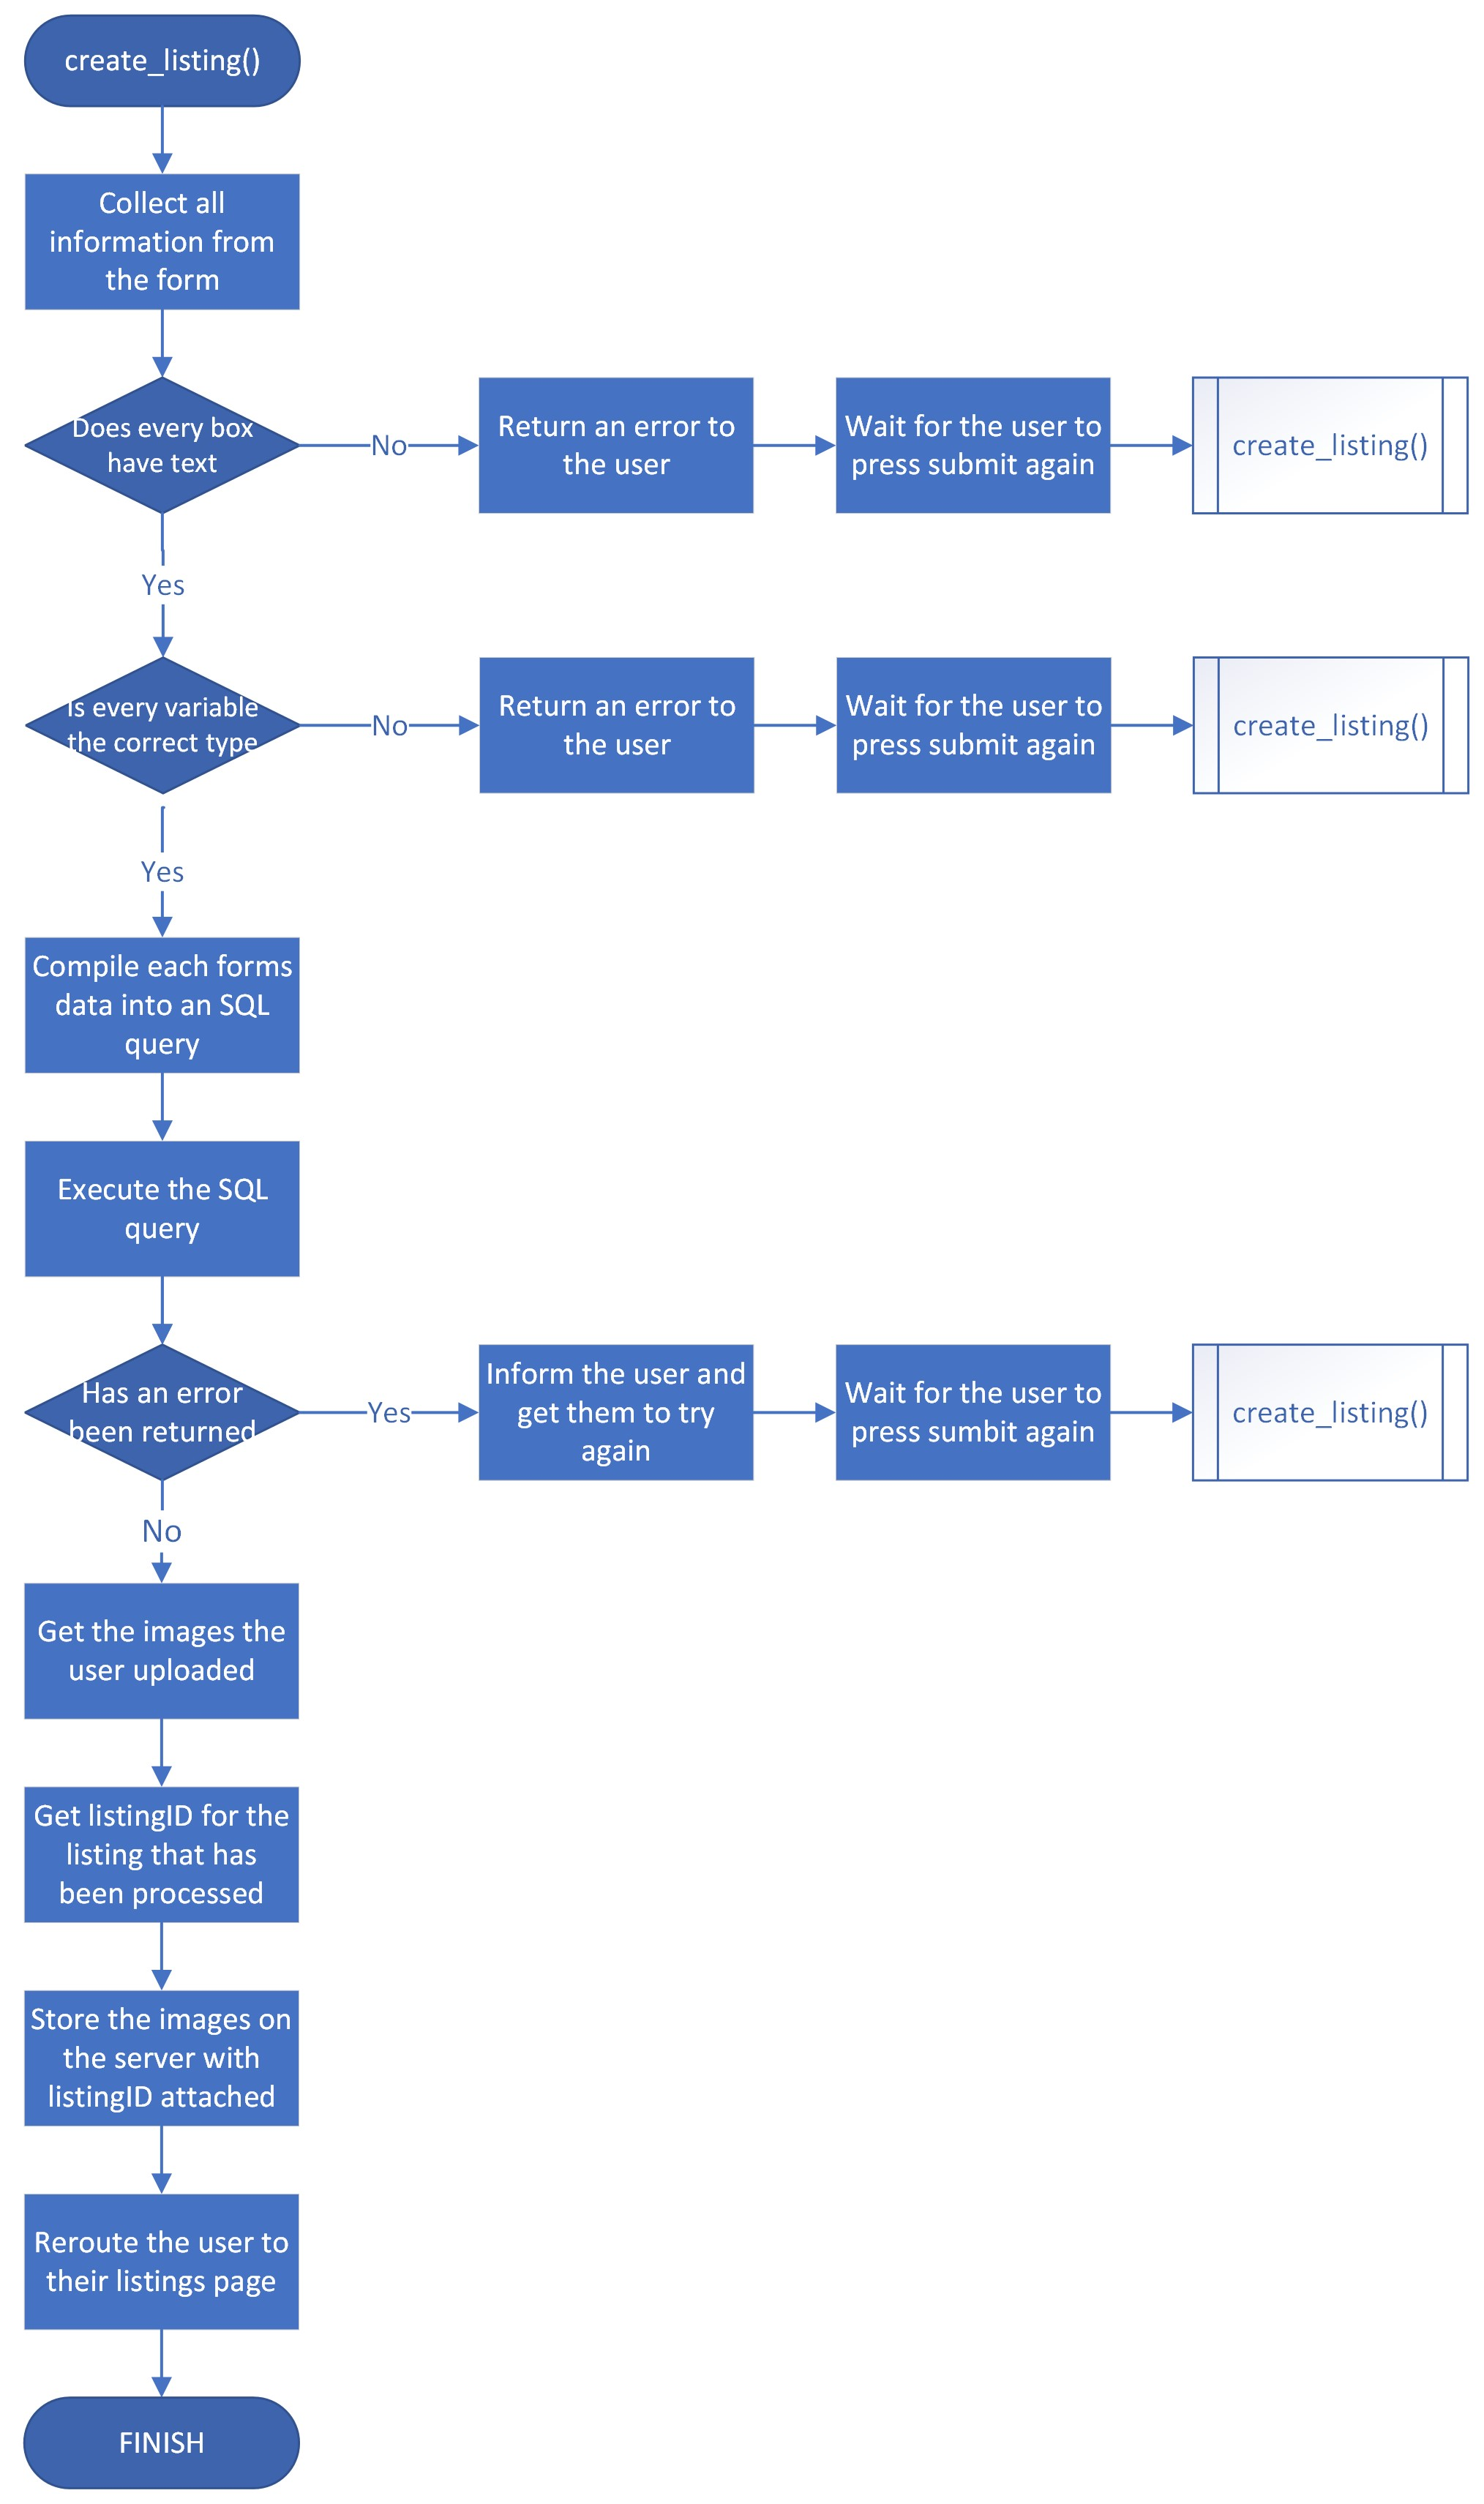
\includegraphics[scale=0.3]{ch2_design/c3_createlisting2.jpeg}
     \caption{Flowchart for the create listing sub-process}
     \label{fig:flow_create}
 \end{figure}
 The process first has to ensure that the actual information has been collected from the form itself which serves as a prerequisite for the rest of the diagram. The next two decisions ensure that the text will not cause any issues if it is entered into the database as ensuring that actual numbers entered will ensure that the database does not return an error. Should the two decisions be approved, then the data can be compiled all together into a single query to go to the listings database, within this process, a listing ID is automatically assigned. By then checking if the query returned an error, it means that we can guarantee that when it comes to adding the images, there will be a listing ID available which ensures the smooth running of the site. The rest of the diagram ensures that all the images is collected and any other information that may be needed. This data is then uploaded and then tagged with the listing ID in order to ensure they can be fetched at a later date. 

\subsection{Price recommendation}
\begin{figure}[H]
    \centering
    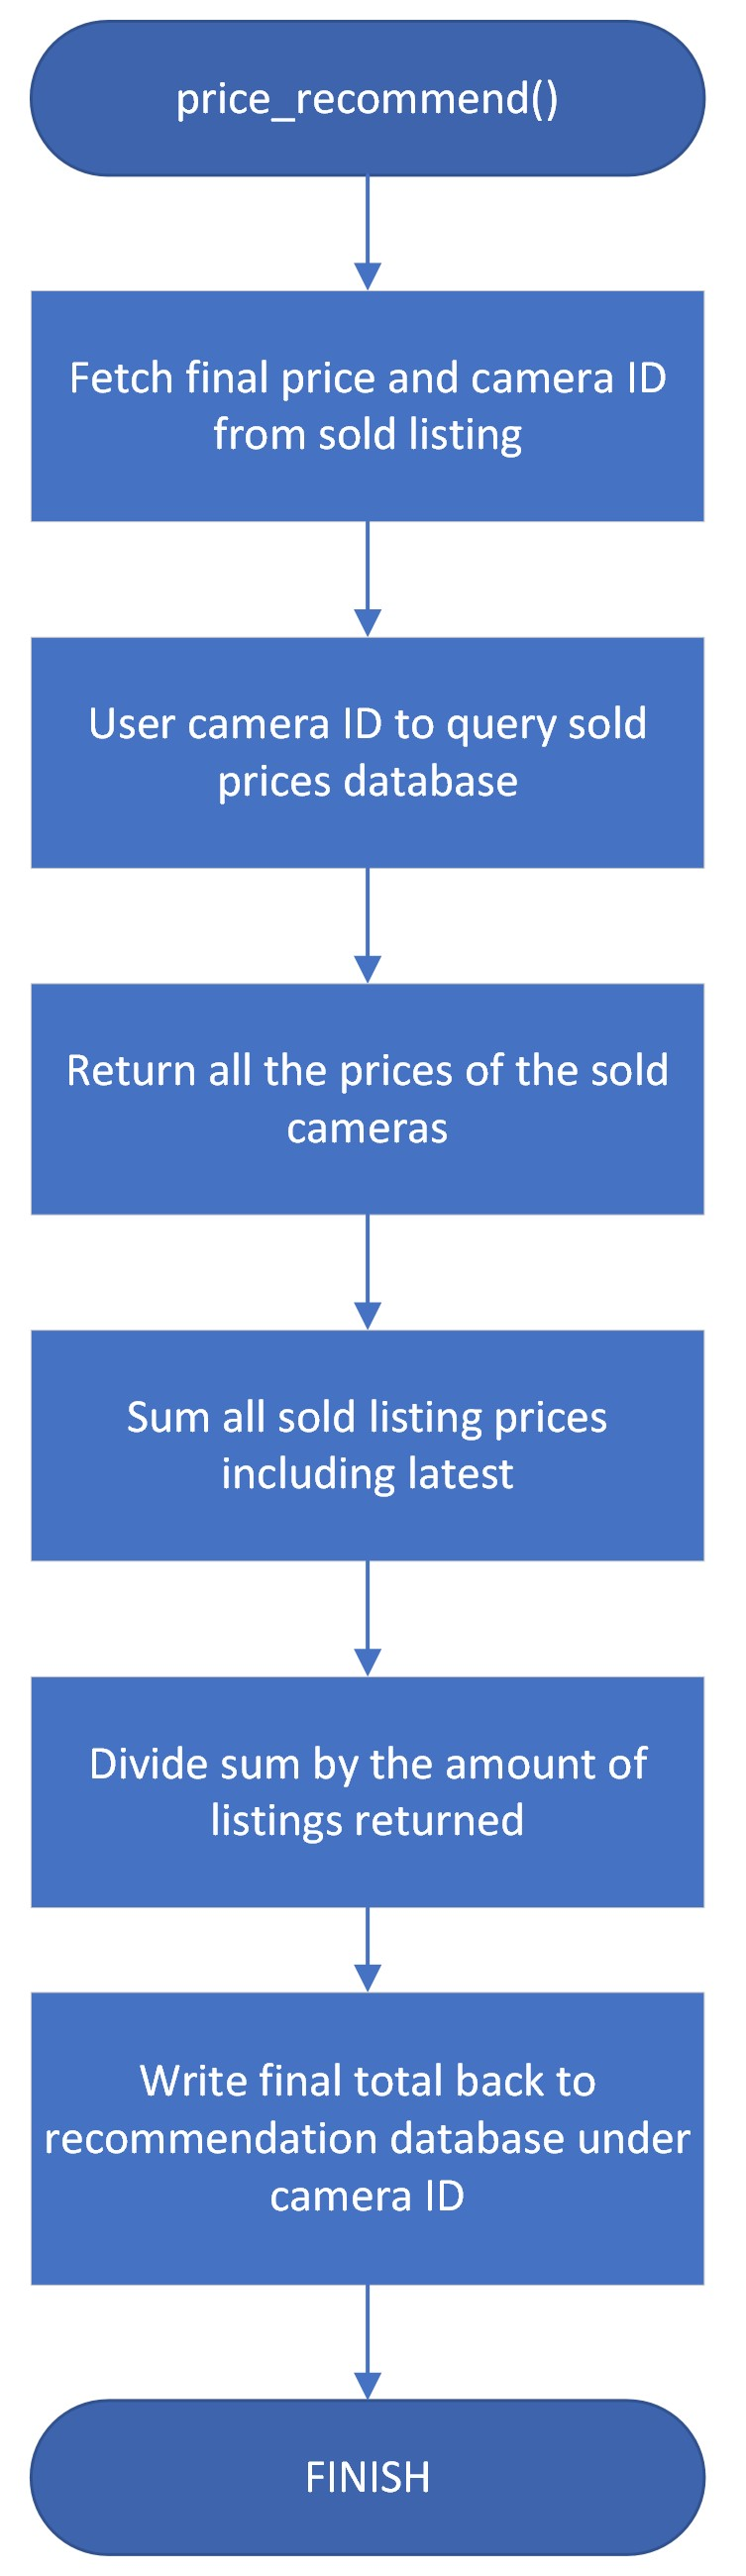
\includegraphics[scale=0.3]{ch2_design/c3_price.jpeg}
    \caption{Flowchart for the price recommendation algorithm}
    \label{fig:flow_price}
\end{figure}
The flowchart will aim to be ran after every listing finishes. It collects the data that will be needed including the camera ID which serves as the primary key for the price recommendation column in order to avoid any issues. A simple mean is performed before all the data is written back to the database with the camera ID being once again used as the primary key for the data.

\subsection{User bidding on a listing}
\begin{figure}[H]
    \centering
    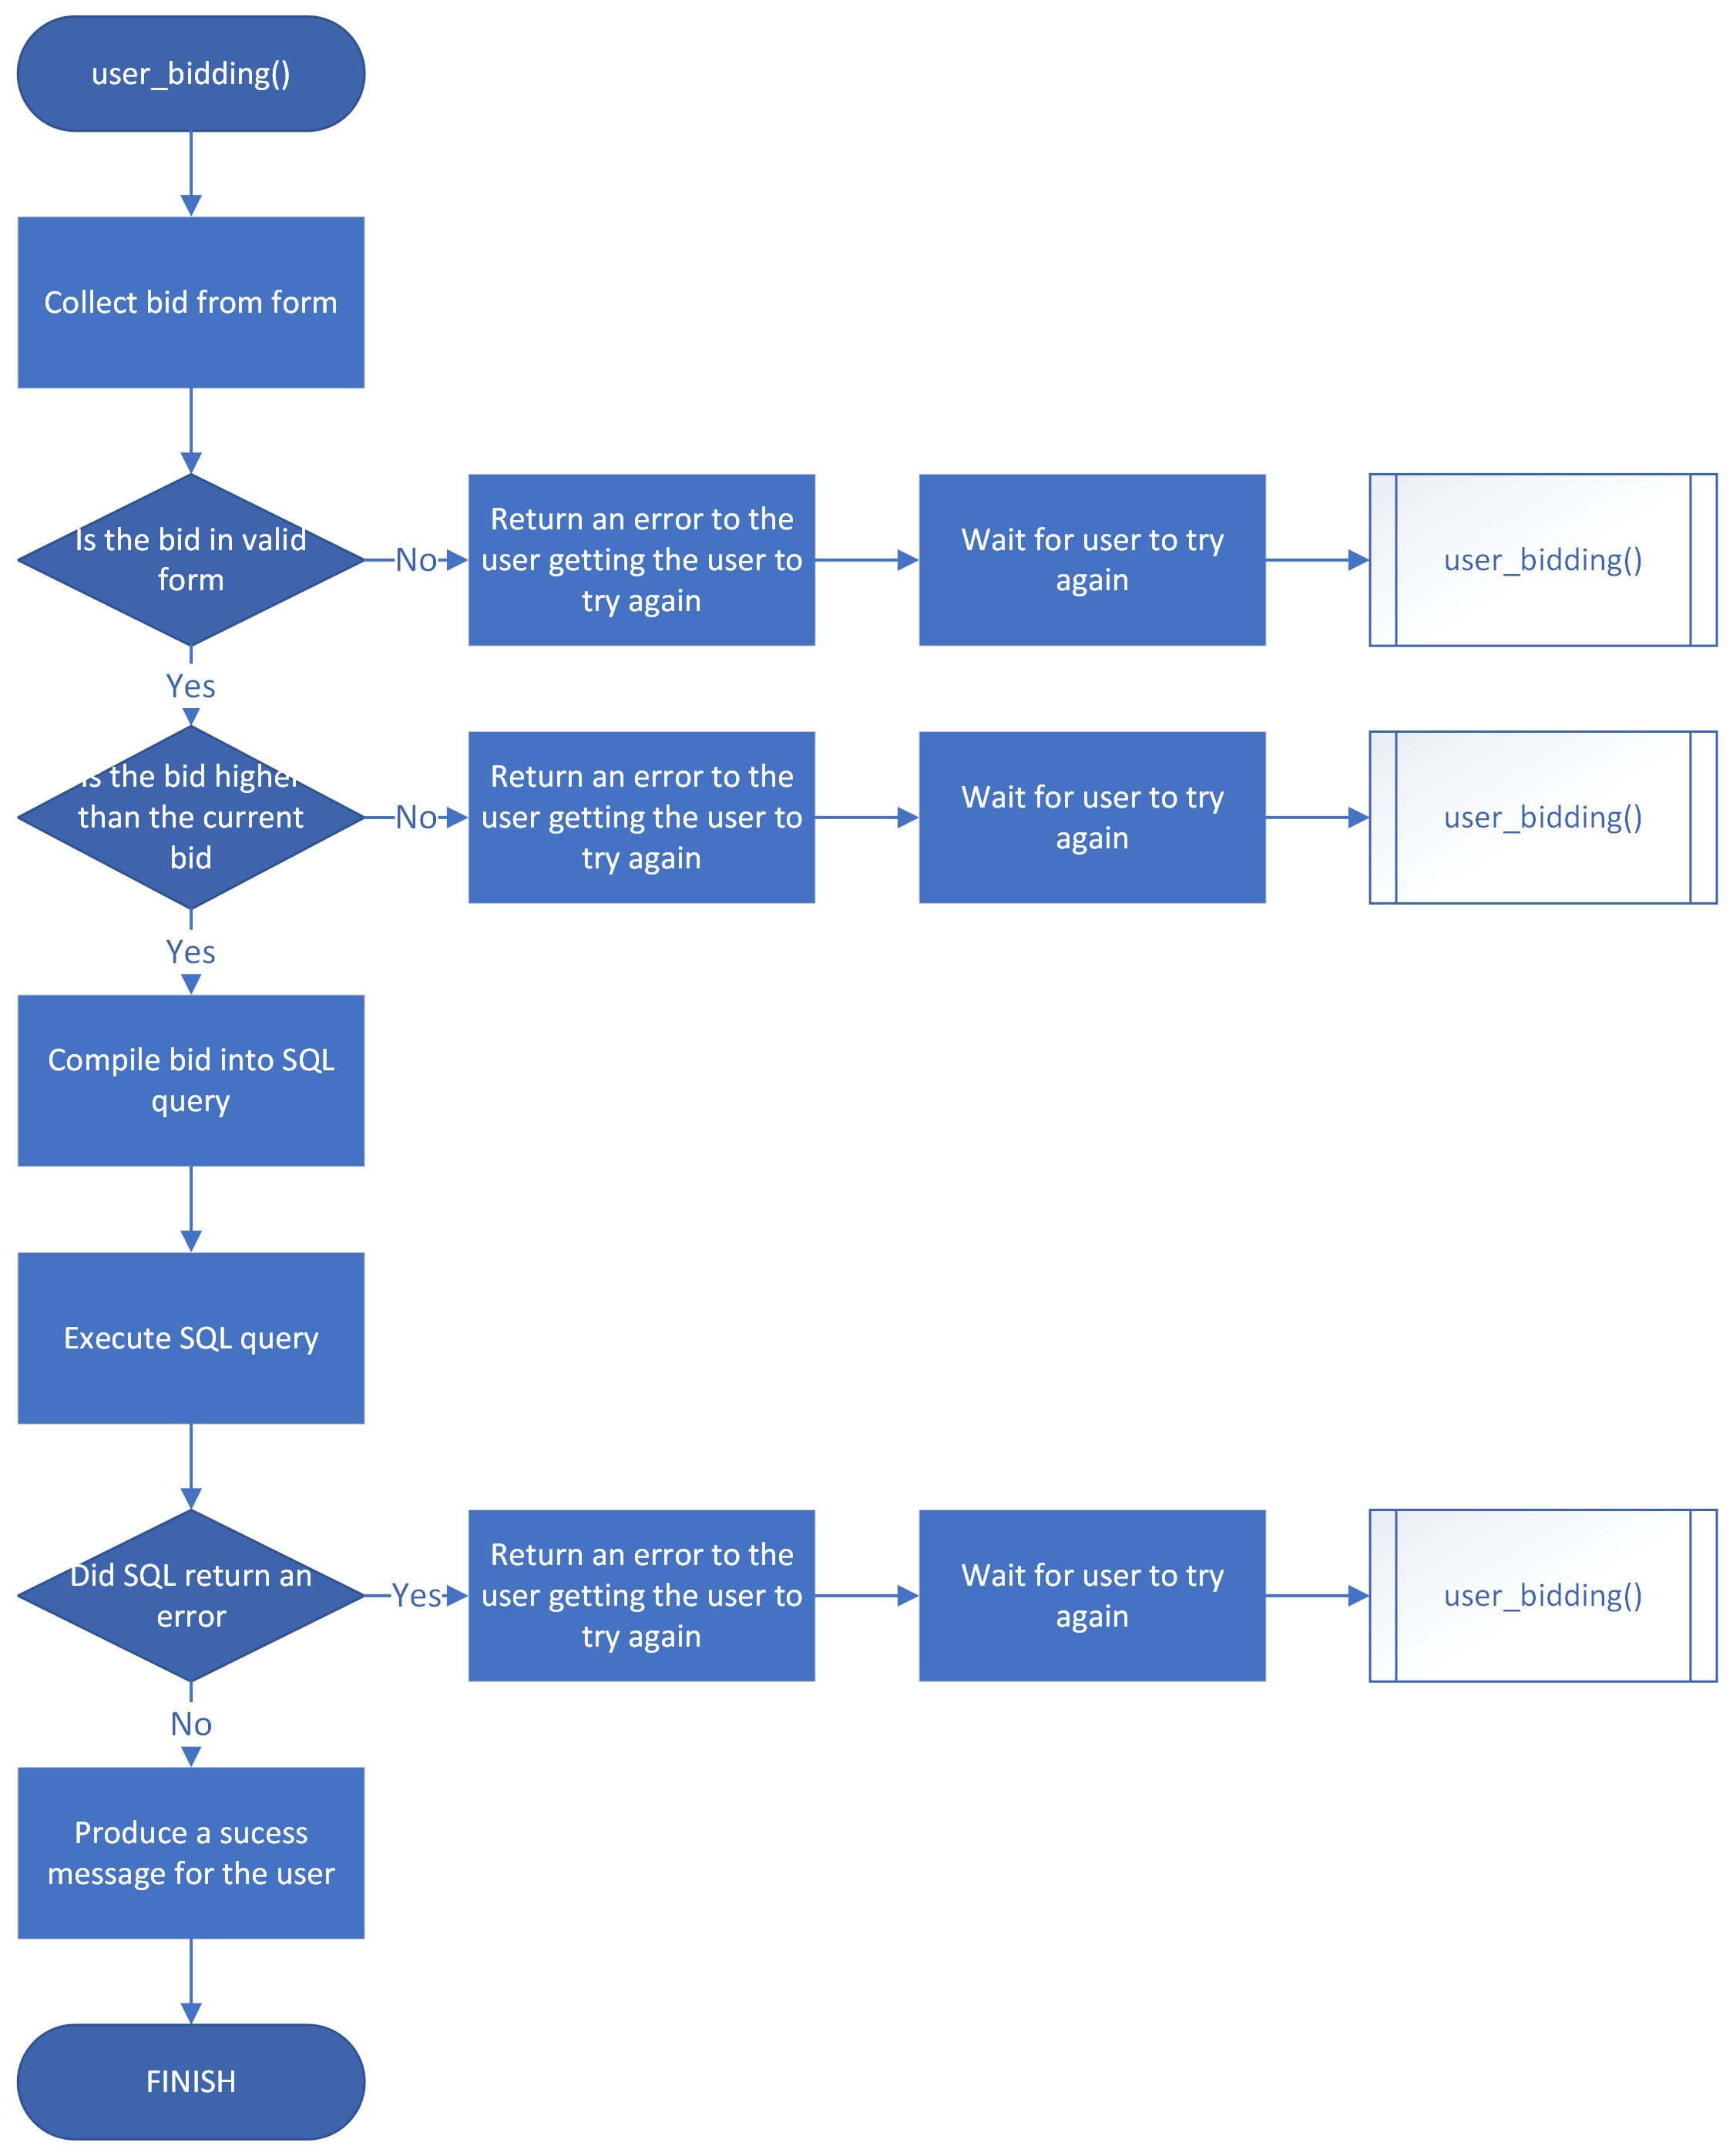
\includegraphics[scale=0.3]{ch2_design/c3_bidding2.jpeg}
    \caption{Flowchart for the process of confirming a user’s bid}
    \label{fig:flow_bidding}
\end{figure}
The process first ensures that data is in the correct format for the variable before the procedure proceeds. This is to make sure that across the rest of the function can run smoothly. The checking of the highest bidder is to ensure that the bid is a valid one and to check the user is not trying to break the site. Both previous tests, culminate with sending a user an error and getting the user to try again so not to discourage them about the usability of the site. By then going on to check the SQL was executed properly, it means that the winning bidder is always the rightful one. 


\subsection{Listing ending}
\begin{figure}[H]
    \centering
    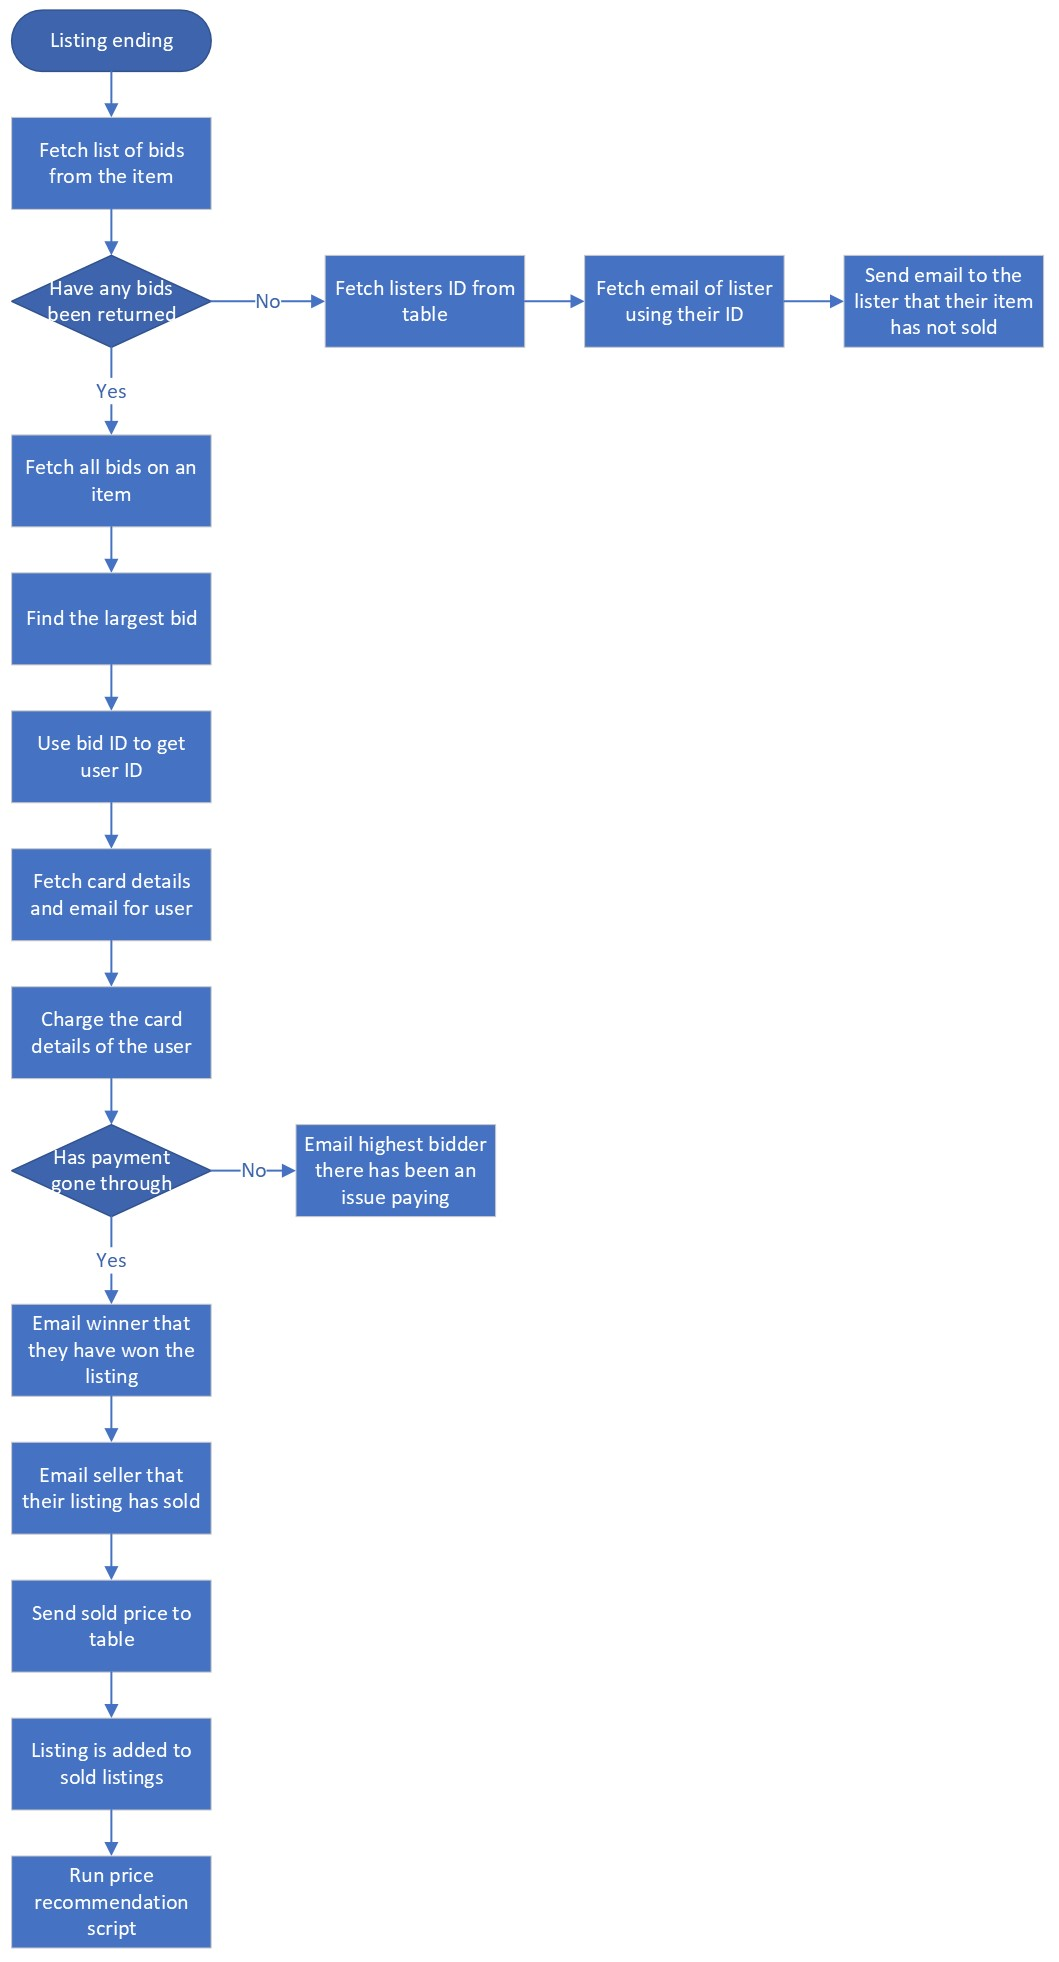
\includegraphics[scale=0.3]{ch2_design/c3_ending.jpeg}
    \caption{Flowchart for the process of when a listing ends}
    \label{fig:flow_ending}
\end{figure}
The process first must check that the item actually has bids on it. This is to ensure that throughout the rest of the flowchart, there will be bids to reference and information to move to different tables. The next steps are to get the details of the user so that they can pay for the item that they have won. It was decided to check that the payment went through properly before sending any information to the seller in order to ensure that a listing is payed for when the email is sent, this eliminates the possibility of a false safe for the seller which also avoids the hassle of re-listing an item. The same methodology of having to possibly re-list in the event of a sale not working applies to the process of moving a sold listing after payment has been completed. 

\section{Project variables}
\begin{center}
\begin{longtable}{|P{1.7cm}|P{1cm}|P{3.5cm}|P{3cm}|P{3cm}|}
  \hline
  \textbf{Variable name} & \textbf{Type} & \textbf{Expected} & \textbf{Justification} & \textbf{Validation} \\
  \hline
  \endfirsthead
  \hline
  \textbf{Variable name} & \textbf{Type} & \textbf{Expected} & \textbf{Justification} & \textbf{Validation} \\
  \hline
  \endhead
  \hline 

  \endfoot
  \endlastfoot
  
    uname & String & Text with simply numbers and characters & Ensures that the website has collected the entered username so that the user can enter the site & Check that the string contains just characters and numbers and check the length to ensure it’s not too long \\ \hline
        psswd & String & A string comprising of numbers and characters including special ones & The password is required in order to make sure that the user can access the site and ensures the form is collecting the data & Check that the password does not contain any spaces \\ \hline
        email & String & Text with no special characters and a ‘@’ symbol & The email is required for site functionality in order to contact the winner of an auction & Ensure that a ‘@’ is present and a domain is at the end such as .com \\ \hline
        card\_number & Int & A 16 digit number with no spaces & The card number is needed to charge the winner & Make sure it only contains numbers and is of the correct length with no spaces \\ \hline
        expiry\_date & DATE & A date in the format year-month & The date must be in that form in order to not cause an error in the SQL database & Check the format of the date in order to see if it could be valid and only contains the year and month \\ \hline
        cvc & Int & A 3 digit security number & The cvc is required in order to charge the user and the payment will not work if the cvc is incorrectly entered & Check that a number has been entered and is a 3 digit number \\ \hline
        Userid & Int & 2/3 digit number unique to the user & The userid ties the listing to a user which enables them to be contacted & Database generated however check if a number has been returned for safety \\ \hline
        Date1 & Int & The current date when the user is using the website & The current date is required in order to create a time left on the listing & Formatted by PHP so no issues \\ \hline
        Date2 & Int & A date in the format year-month-date returned from the database & The second date is required to calculate the interval for the listing & The date is verified before it is sent to the database so shouldn’t be any alternation whilst in the table \\ \hline
        Interval & Int & The interval between the two date variables & The interval is required to in order for the user to see how long is left on the listing and in order to remove listings when the time has expired & Check that the result that has been retuned is a positive interval by being greater than 0 \\ \hline
        Search & String & A make and/or model of a camera that the user wants to search for & A key aspect of the site and therefore has to receive the right data & Check that the string does not contain any special characters that wouldn’t be found in a camera model \\ \hline
        listingID & Int & The unique 2/3 digit code for a listing & The listingID allows all the information to be returned by the site for the listing that the user has specified when they view the listing & The ID is generated by the database when a listing is created and therefore shouldn’t have any issues however check a number has been retuned \\ \hline
        Make & String & A camera brand comprising of just a simple text string with no special characters & The camera brand is needed in order for the user to identify the camera and for users to be able to search for a camera & Check that a string has been returned that contains only basic text with no special characters \\ \hline
        Model & String & The model of a camera should only be characters and numbers & The model is crucial for the user to know what camera they are looking at & Check that the string doesn’t contain anything that is not a number or character \\ \hline
        Price & Float & A possible decimal number however could be an integer & The price is needed in order for the user to know how much they need to bid & Check that the price only contains numbers \\ \hline
        Description & String & Long string that should contain information on the camera & The description allows the user to better understand what camera they are going to be getting & Check the length of the description in order to ensure some text has been written and the box therefore is not blank \\ \hline
        End\_date & Int & Holds the date that the listing will end & This allows the listing to run out of time in order to conform to an auction style format & The formatting is handled by php however check that a date has indeed been entered \\ \hline
    \caption{Development variable table}
\label{tab:develop_var}
\end{longtable}
\end{center}

\section{Algorithms \parencite{carbon_app}}
\subsection{Login page}
\begin{figure}[H]
    \centering
    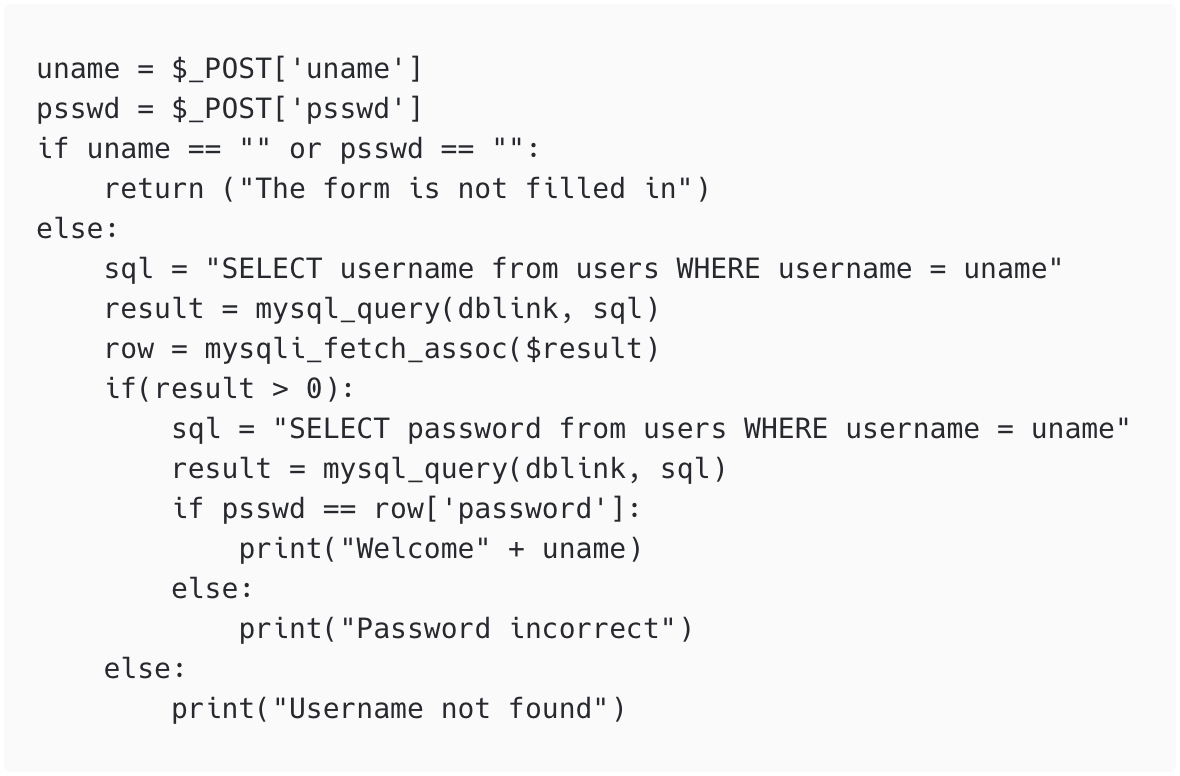
\includegraphics[scale=0.4]{ch2_design/alg_login.png}
    \caption{Pseudocode for the user to log into the site}
    \label{fig:alg_login}
\end{figure}
The code follows the procedure outlined in the previous flow diagram. It aims to first ensure that the user has entered text into the form through the user of a basic if statement. The following collection of nested if and else statements first checks that at username can be found. This is achieved through creating an SQL statement before executing it. The first statement only contains the username as to ensure we only see if that username exists. The result variable that is used multiple times allows us to hold all the information that has been fetched from the external database. Once the username has been established to be in the system, another SQL statement is executed this time fetching the password in order to carry out a comparison to check the right details have been entered. If all the details are correct, the user is forwarded to the home page after being greeted by a message that contains the user’s username.

\subsection{Sign-up page}
\begin{figure}[H]
    \centering
    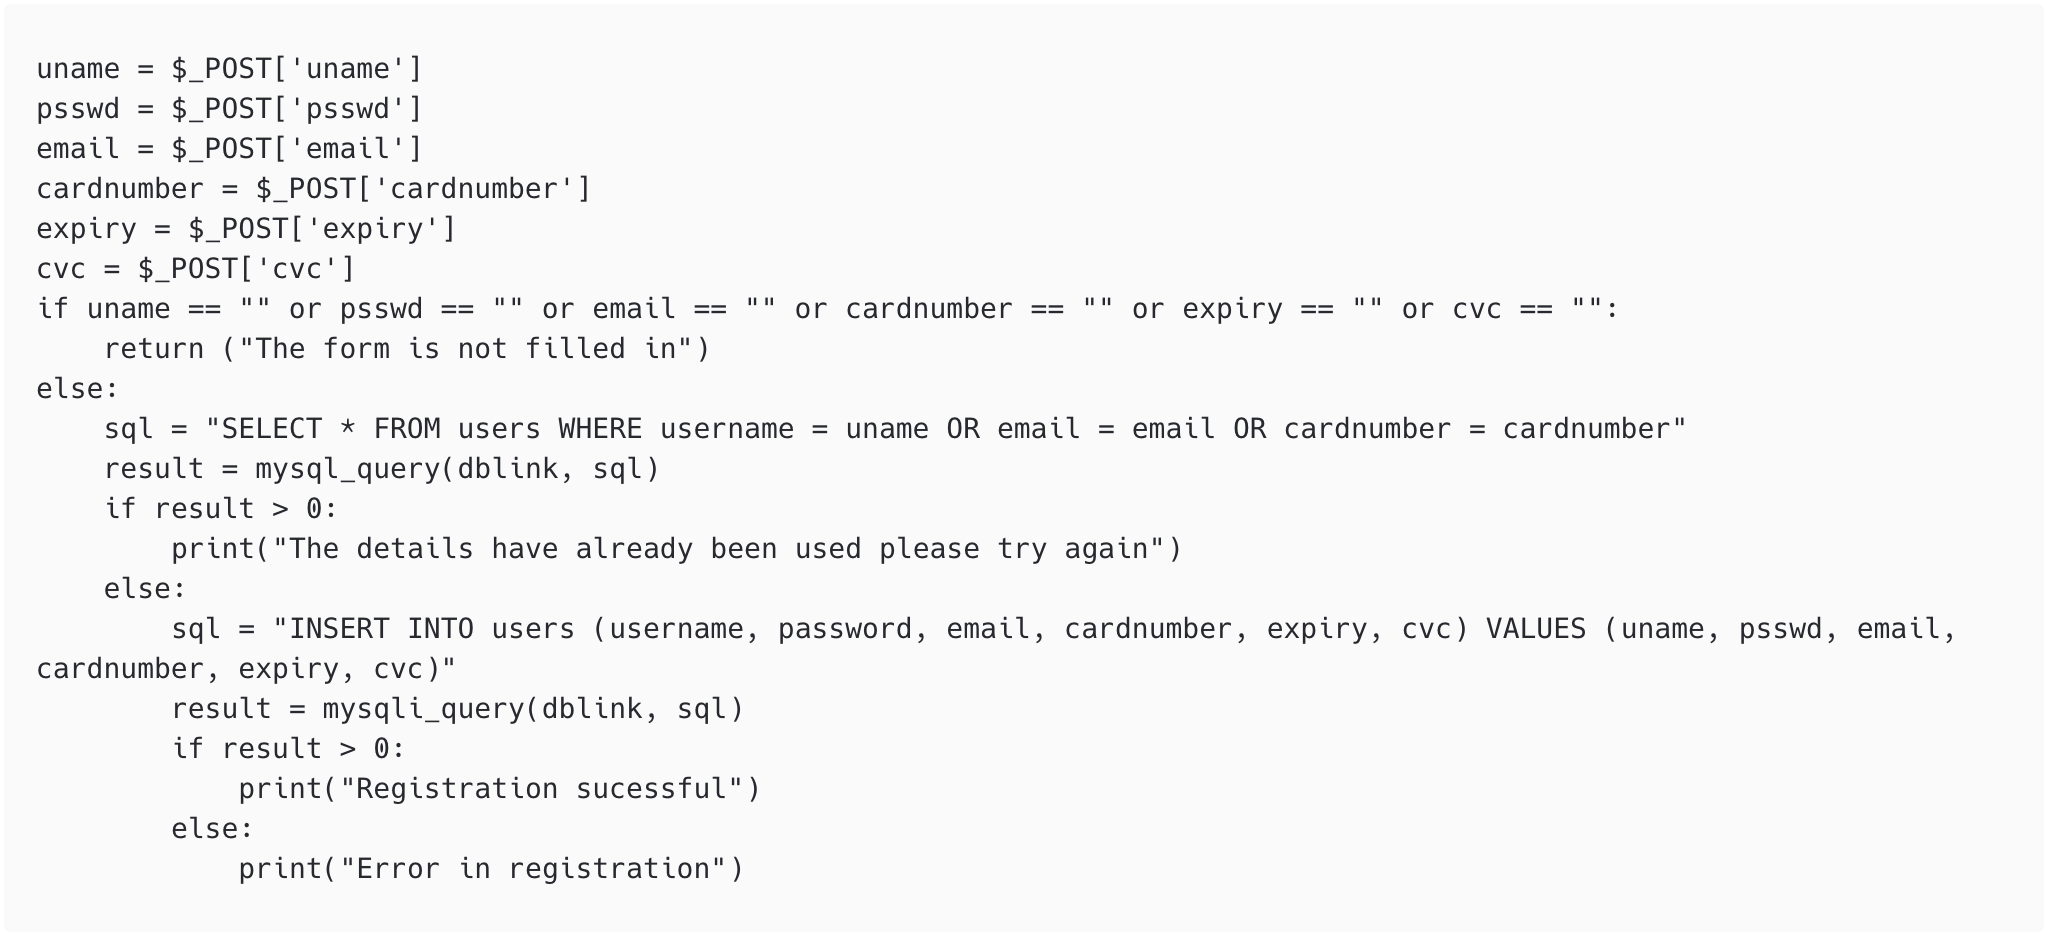
\includegraphics[scale=0.2]{ch2_design/alg_signup.png}
    \caption{Pseudocode to register for the website}
    \label{fig:alg_signup}
\end{figure}
The code works to first collect the information from the websites form and covert it to variables that can be used throughout the code. An if statement then checks to see if the form did contain all the data that it needed to. This ensures the smooth running of the page. The form data is then used to query the database in order to check that it is unique, if results are returned by the query, then we know that the data is already entered by another user. If the registration hasn’t failed, it will then insert the all the form data into the database. If all executes without error, the user is forwarded onto the main home page.
 
\subsection{Searching for a listing}
 \begin{figure}[H]
     \centering
     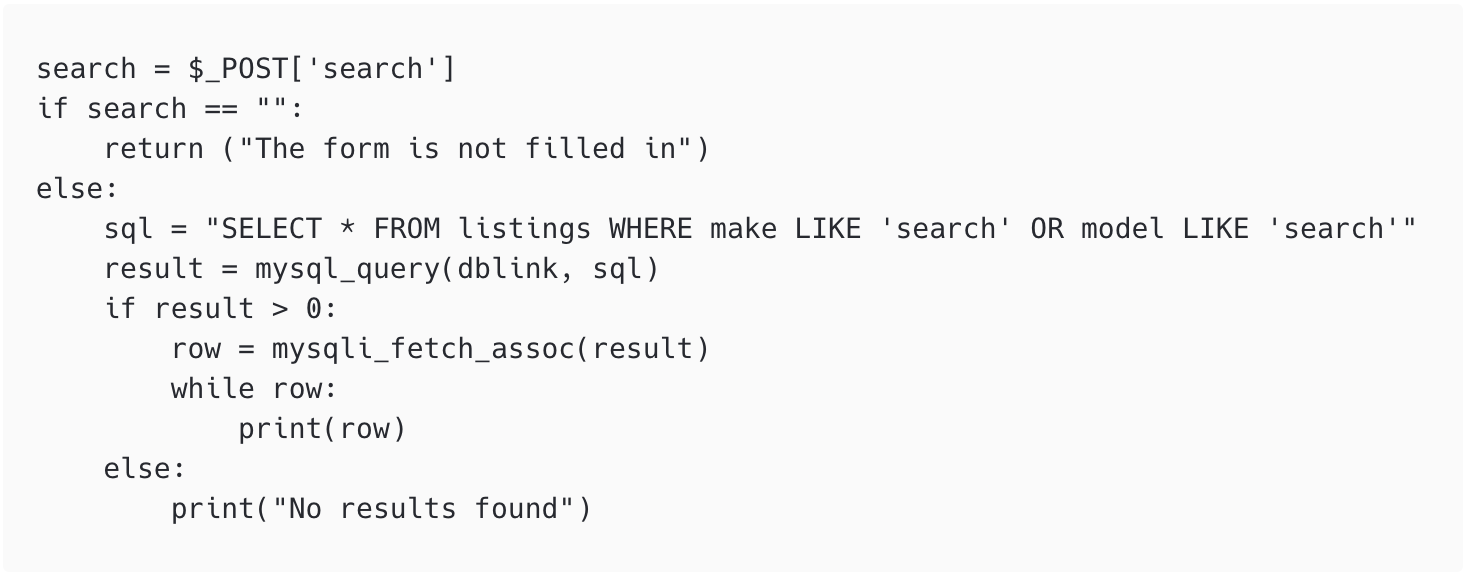
\includegraphics[scale=0.3]{ch2_design/alg_search.png}
     \caption{Pseudocode to search for a listing}
     \label{fig:alg_search}
 \end{figure}
The code first compiles an SQL query that will search the listings database for a camera with the make and model that is similar to that which the user has entered. The code then ensures that the query has returned results. In the case that it hasn’t found any listings of the description, it will return an error to the user that nothing has been found. If results are found, then the code will cycle through all the results that have been returned using a while loop. For each of the rows that have been returned, the information is outputted with the images being found through searching with the file name that is stored in the database. A view listing button is also there which will link to the next page using the lisitngID.

\subsection{Creating a listing}
\begin{figure}[H]
    \centering
    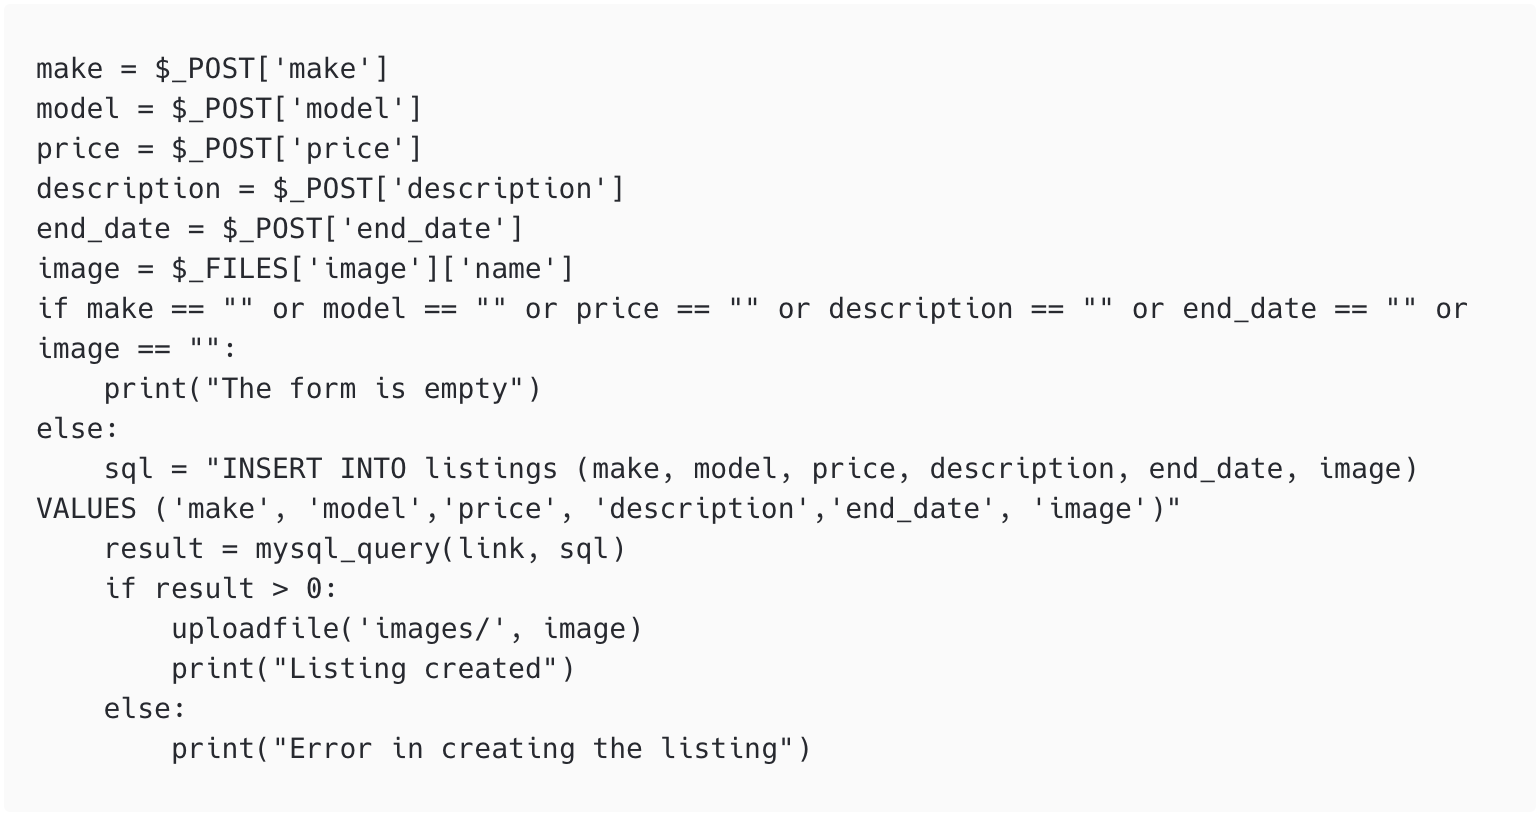
\includegraphics[scale=0.3]{ch2_design/alg_creating.png}
    \caption{Pseudocode to create a listing}
    \label{fig:alg_creating}
\end{figure}
The algorithm first aims to define the SQL statement that is needed to be executed on the database. It works to collect the information from the form on the webpage. This also includes the user’s username which is sent in order that the listing can be identified. First checking that the SQL query worked, the image that the user added to the listing will also now be saved to the server. The program will return an error message either way that the code executes. 

\subsection{Price recommendation}
\begin{figure}[H]
    \centering
    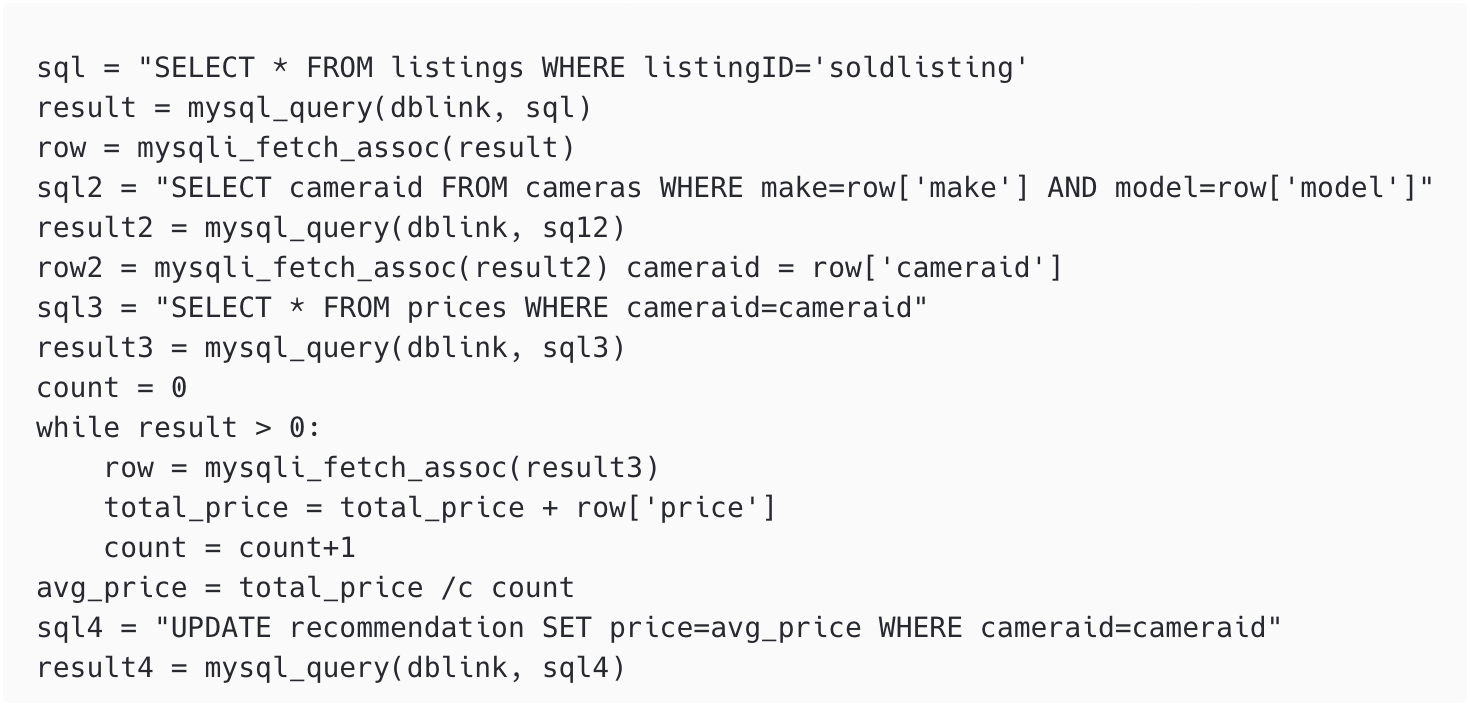
\includegraphics[scale=0.3]{ch2_design/alg_price.png}
    \caption{Pseudocode in order to update the recommendation price}
    \label{fig:alg_price}
\end{figure}
The code will first collect all the information about the listing from the database, this is so that the make and model can be used to query the cameras database. The make and model are used to retrieve the cameras id number. This is so that all the sold prices can be used. The algorithm will then fetch all the prices from the system and add them all up. At the same time, it is so keeping count of how many prices for that camera have been found in order to perform an average at the end. The average value is then found through taking the total value and dividing it by the count. This value is then sent to the database.  

\subsection{User bidding on an item}
\begin{figure}[H]
    \centering
    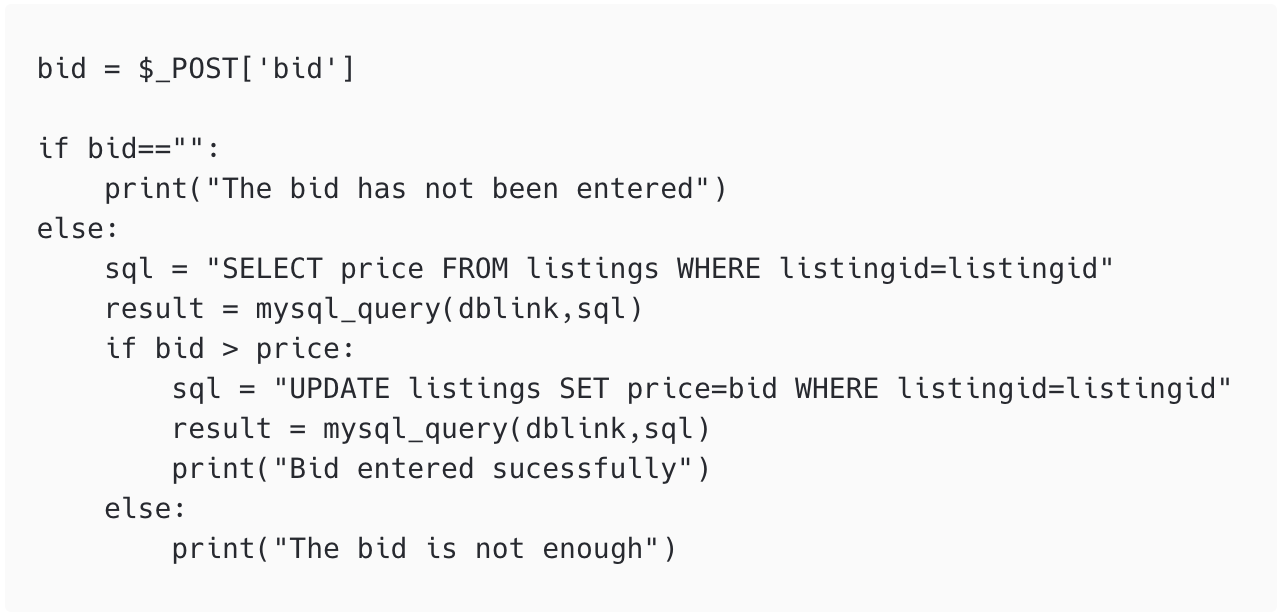
\includegraphics[scale=0.3]{ch2_design/alg_bid.png}
    \caption{Pseudocode for the algorithm for the user to bid on an item}
    \label{fig:alg_bid}
\end{figure}
The bid is first collected from the website form and is checked that it contains a value in order to best ensure the running of the site. If there is an issue, then the user is given an error and else is allowed to continue. The SQL statement is then defined and executed; this is with the aim of getting the current price of the listing. The price that has been fetched is compared to the one that has been entered and providing the bid is greater than the current price then the new bid is added to the database and becomes the price of the listing. If the bid is not enough then an error is returned. 
 
\section{Tests for prototype 1}
For prototype 1, I’m focussing the tests in order to establish which parts of the program are working as intended and which parts require further development. To achieve this, I will use three types of tests: normal, erroneous and boundary. Normal tests are the intended function of the program and work to check that the code I’ve wrote will execute as intended. Erroneous tests are tests that are designed to break the program. This allows me to test verification algorithms and see which forms are missing validation. I have used boundary testing sparingly to reduce testing time. Boundary tests are long inputs that are used to test the program can handle long inputs. PHP and MySQL are both equipped to deal with long inputs and so are expected to handle this part of the program well. 
\begin{center}
\begin{longtable}{|P{3cm}|P{1.7cm}|P{3cm}|P{2.6cm}|P{2cm}|}
  \hline
  \textbf{Test} & \textbf{Type} & \textbf{Expected result} & \textbf{Actual result} & \textbf{Evidence} \\
  \hline
  \endfirsthead
  \hline
  \textbf{Test} & \textbf{Type} & \textbf{Expected result} & \textbf{Actual result} & \textbf{Evidence} \\
  \hline
  \endhead
  \hline 

  \endfoot
  \endlastfoot

  Can the user enter a username & Normal & The user can enter a username into the login & ~ & ~ \\ \hline
        Can the user enter a password & Normal & The user can enter a password into the box & ~ & ~ \\ \hline
        Can the user enter an email & Normal & The user can enter an email into the box & ~ & ~ \\ \hline
        Can the user enter their card number & Normal & The user can enter 16 digits for a card number & ~ & ~ \\ \hline
        Can the user enter their expiry & Normal & The user can enter a month and year into the box & ~ & ~ \\ \hline
        Can the user enter their cvc & Normal & The user can enter a 3-digit number into the box & ~ & ~ \\ \hline
        Does the username get checked its unique & Normal / Erroneous & The database is queried and if results are returned then an error is returned to the user & ~ & ~ \\ \hline
        Does the email get check that it is unique & Normal / Erroneous & Database queried and if results are returned then an error is returned & ~ & ~ \\ \hline
        Does the card number get checked to be unique & Normal / Erroneous & Database queried and if results are returned give the user an error & ~ & ~ \\ \hline
        If the user if logging in is their username checked to see if it exists & Normal / Erroneous & Database is queried to see if a result is returned & ~ & ~ \\ \hline
        If the user is logging in is the password checked against the username in the database & Normal / Erroneous & Database queried with username to see whether the password returned matches one entered & ~ & ~ \\ \hline
        When logging in if the user enters a username that does not exist are they given an error & Erroneous & Give an error if the database doesn’t return any results & ~ & ~ \\ \hline
        When logging in if the username and password do not match is an error returned & Erroneous & The database is queried, if a password is returned that doesn’t match then return an error & ~ & ~ \\ \hline
        Is a search button on the home page & Normal & Button on homepage & ~ & ~ \\ \hline
        Is a create a listing button on the home page & Normal & Button on homepage & ~ & ~ \\ \hline
        Is a price recommendation button on the homepage & Normal & Button on homepage & ~ & ~ \\ \hline
        Can the user enter a camera on the search page & Normal & The user can enter text into the box & ~ & ~ \\ \hline
        Does the camera entered get used as a search term for the database & Normal & Does the term get used in the SQL query & ~ & ~ \\ \hline
        Are results returned if a valid result is entered & Normal & Results are outputted on the page & ~ & ~ \\ \hline
        If nothing is entered in the search bar is an error returned & Erroneous & Error returned to the user & ~ & ~ \\ \hline
        Can the user click the view button on a search result and view the listing & Normal & The user is forwarded to the listing’s page & ~ & ~ \\ \hline
        If the user does not enter text in a box is an error returned & Erroneous & The user is given an error saying the report is incomplete & ~ & ~ \\ \hline
        If the user doesn’t upload an image is an error returned & Erroneous & The user is told an image has not been added & ~ & ~ \\ \hline
        Is an error returned if an image is not uploaded & Erroneous & The user is given a error detailing that not a valid file type has been entered & ~ & ~ \\ \hline
        If the user enters a bid too low on the listing is an error returned & Erroneous & The user is told the bid is not enough & ~ & ~ \\ \hline
        If the user enters a really large bid, does it still process & Boundary & Bid processes normally & ~ & ~ \\ \hline
        If the user enters a bid with lots of zeros it treated normally & Boundary & The bid is treated normally & ~ & ~ \\ \hline
        If the user enters a higher bid, then does it get processed & Normal & Bid goes through and all is updated at the database end & ~ & ~ \\ \hline

    \caption{Test plan for prototype 1}
\label{tab:proto1_test_plan}
\end{longtable}
\end{center}